\documentclass[UTF8,a4paper,12pt]{ctexbook} 

\usepackage{graphicx}%学习插入图
\usepackage{verbatim}%学习注释多行
\usepackage{booktabs}%表格
\usepackage{geometry}%图片
\usepackage{amsmath}
\usepackage{amssymb}
\usepackage{listings}%代码
\usepackage{xcolor}  %颜色
\usepackage{enumitem}%列表格式
\setenumerate[1]{itemsep=0pt,partopsep=0pt,parsep=\parskip,topsep=5pt}
\setitemize[1]{itemsep=0pt,partopsep=0pt,parsep=\parskip,topsep=5pt}
\setdescription{itemsep=0pt,partopsep=0pt,parsep=\parskip,topsep=5pt}
\usepackage{tcolorbox}
\usepackage{algorithm}  %format of the algorithm
\usepackage{algorithmic}%format of the algorithm
\usepackage{multirow}   %multirow for format of table
\usepackage{tabularx} 	%表格排版格式控制
\usepackage{array}	%表格排版格式控制
\usepackage{hyperref} %超链接 \url{URL}
\usepackage{tikz}
\usepackage{dirtree}


\usetikzlibrary{intersections,
	positioning,
	petri,
	backgrounds,
	fit,
	decorations.pathmorphing,
	arrows,
	arrows.meta,
	bending,
	calc,
	intersections,
	through,
	backgrounds,
	shapes.geometric,
	quotes,
	matrix,
	trees,
	shapes.symbols,
	graphs,
	math,
	patterns,
	external}
\CTEXsetup[format+={\flushleft}]{section}

%%%% 设置图片目录
\graphicspath{{figure/}}

%%%% 段落首行缩进两个字 %%%%
\makeatletter
\let\@afterindentfalse\@afterindenttrue
\@afterindenttrue
\makeatother
\setlength{\parindent}{2em}  %中文缩进两个汉字位

%%%% 下面的命令重定义页面边距,使其符合中文刊物习惯 %%%%
\addtolength{\topmargin}{-54pt}
\setlength{\oddsidemargin}{0.63cm}  % 3.17cm - 1 inch
\setlength{\evensidemargin}{\oddsidemargin}
\setlength{\textwidth}{14.66cm}
\setlength{\textheight}{24.00cm}    % 24.62

%%%% 下面的命令设置行间距与段落间距 %%%%
\linespread{1.4}
\setlength{\parskip}{0.5\baselineskip}
\geometry{left=1.6cm,right=1.8cm,top=2cm,bottom=1.7cm} %设置文章宽度
\pagestyle{plain} 		  %设置页面布局

%代码效果定义
\definecolor{mygreen}{rgb}{0,0.6,0}
\definecolor{mygray}{rgb}{0.5,0.5,0.5}
\definecolor{mymauve}{rgb}{0.58,0,0.82}
\lstset{ %
	backgroundcolor=\color{white},   % choose the background color
	basicstyle=\footnotesize\ttfamily,      % size of fonts used for the code
	%stringstyle=\color{codepurple},
	%basicstyle=\footnotesize,
	%breakatwhitespace=false,         
	%breaklines=true,                 
	%captionpos=b,                    
	%keepspaces=true,                 
	%numbers=left,                    
	%numbersep=5pt,                  
	%showspaces=false,                
	%showstringspaces=false,
	%showtabs=false,        
	columns=fullflexible,
	breaklines=true,                 % automatic line breaking only at whitespace
	captionpos=b,                    % sets the caption-position to bottom
	tabsize=4,
	commentstyle=\color{mygreen},    % comment style
	escapeinside={\%*}{*)},          % if you want to add LaTeX within your code
	keywordstyle=\color{blue},       % keyword style
	stringstyle=\color{mymauve}\ttfamily,     % string literal style
	frame=L,
	xleftmargin = .079\textwidth,
	rulesepcolor=\color{red!20!green!20!blue!20},
	% identifierstyle=\color{red},
	language=c++,
}
 \author{\kaishu 郑华}
 \title{\heiti U3D笔记}
 
\begin{document}          %正文排版开始
 	\maketitle
 	\tableofcontents

\chapter{基础}
	入门参考:\url{https://unity3d.com/cn/learn/tutorials}
	
	\section{如何将脚本与具体对象绑定}
		\begin{enumerate}
			\item 右键\verb|asset|文件夹,创建C\#脚本
			\item 编写脚本
			\item 将\verb|asset |中的脚本拖拽到 \verb|hiearch |视图中的\verb|MainCamera |中
			\item 如果脚本是作用于场景中的某个物体,\textbf{则将该脚本拖拽到该物体上}
		\end{enumerate}
	
	\section{序列化-  [SerializedField]}
		\textit{通常情况下},GameObject上挂的MonoBehaviour脚本中的\textbf{私有变量}\textit{不会显示在Inspector面板上},即不会被序列化。
		
		\textbf{但如果指定了SerializedFiled特性},就可以被序列化了。
		
		\begin{lstlisting}
	public class Test : MonoBehaviour 
	{
		public string Name;
		[SerializeField]
		private int Hp; 
	}
		\end{lstlisting}
		
		\begin{figure}[H]
			\centering
			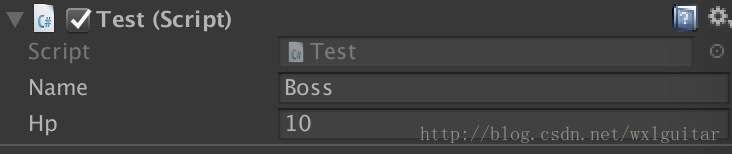
\includegraphics[scale=0.8]{SerilizedFiled.jpg}
			\caption{序列化操作 -在Inspector上显示}
		\end{figure}
	
	\section{常用技巧}
		\begin{itemize}
			\item \verb|ctrl + d| 复制
			\item \verb|shift + 鼠标 | 等比例缩放 
			\item \verb|shift + alt + 鼠标 | 原地等比例缩放
			\item \verb|在Unity 编辑器中输入汉字 | 需要借助其他文本拷贝粘贴
			\item \verb|q、w、e、r、t |在操作UI时尽量使用 T,以避免z轴发生的变化 
		\end{itemize}
	
	\section{MonoBehaviour 生命周期、渲染管线}
		
		\subsection{脚本渲染流程}
			\begin{figure}[H]
				\centering
				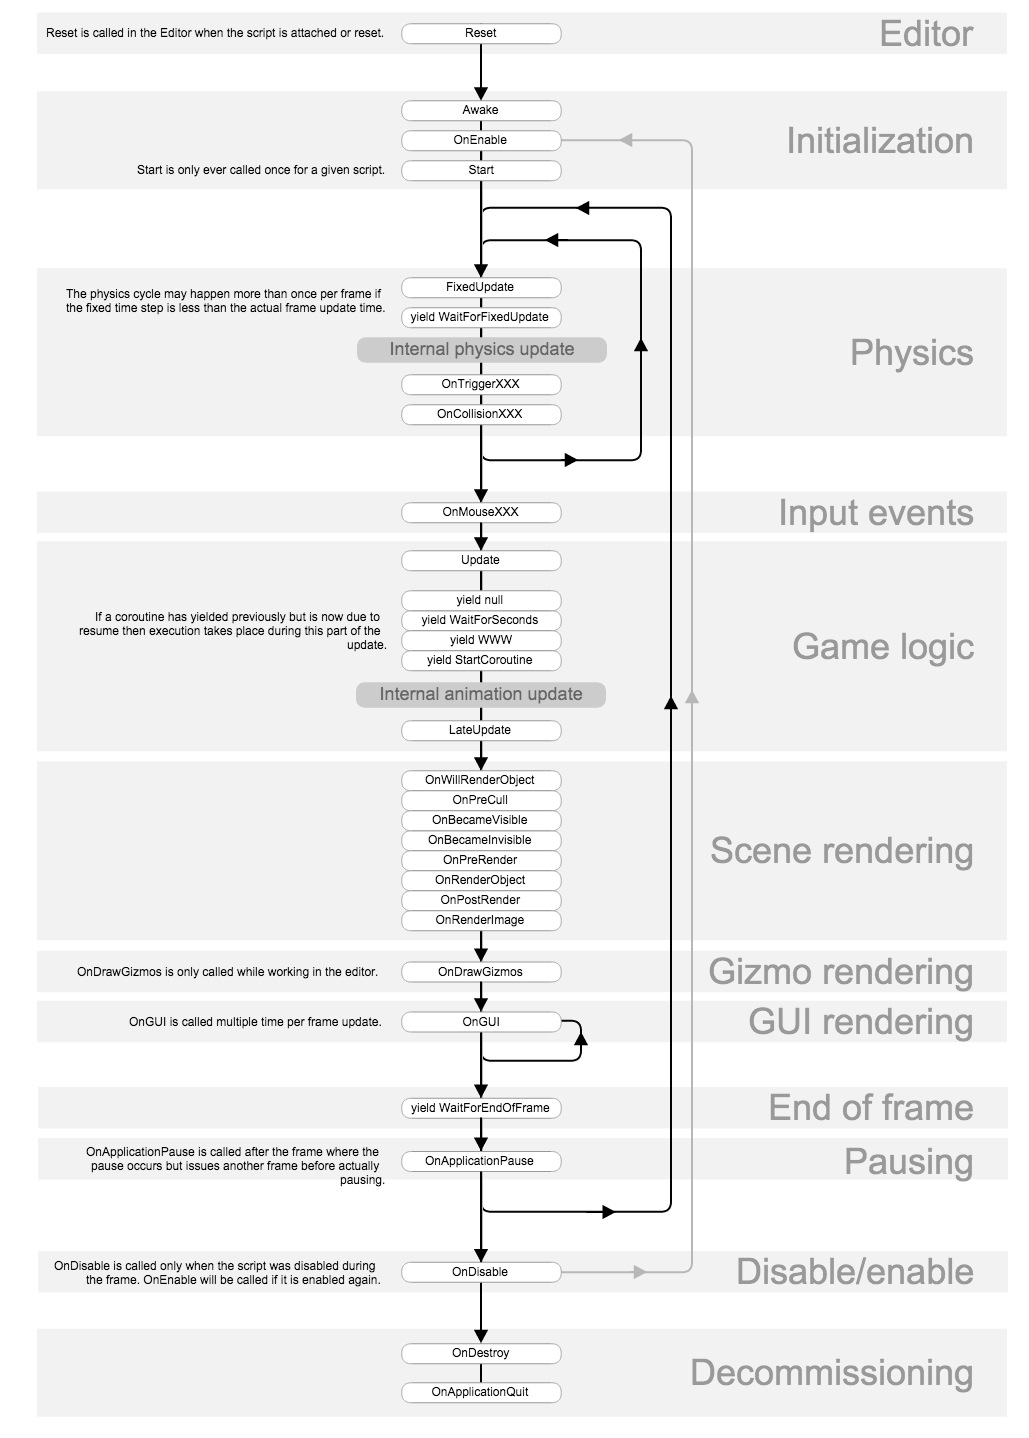
\includegraphics[scale=0.44]{scriptLifeCircle.jpg}
				\caption{脚本生命周期核心方法}
			\end{figure}
			
			\clearpage
			\begin{figure}[H]
				\centering
				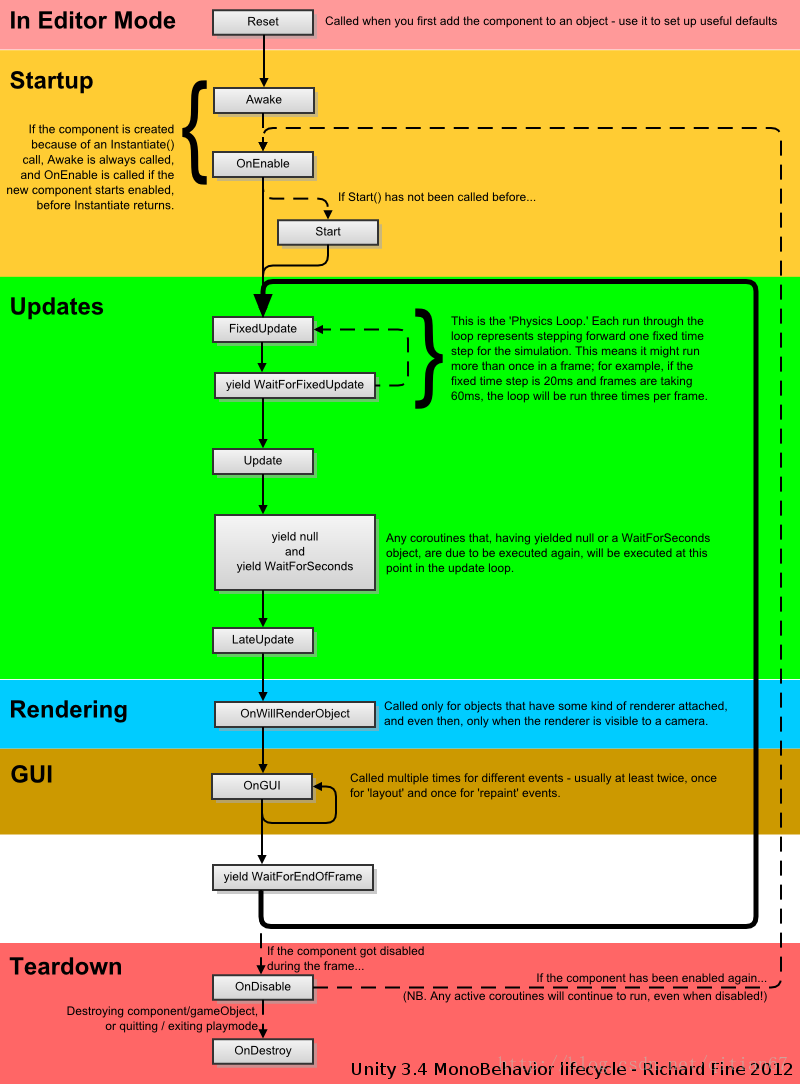
\includegraphics[scale=0.78]{LifeCicle.png}
				\caption{简要核心方法}
			\end{figure}
		
		update:当其\textbf{所在的物体}属于未激活的话(\verb|active为false|),\textit{该物体上所有脚本中包含的协程代码都是不会被执行的}。
		\subsection{核心方法}
			\begin{enumerate}
				\item \verb|Reset |:
				\item \verb|Awake |:脚本唤醒函数,\textbf{当游戏对象被创建的时候},\textit{游戏对象}\textbf{绑定的脚本会在该帧(Frame)内}\textit{执行Awake() 函数},\textbf{无论}脚本是否处于激活(\textbf{enable})状态。
				\item \verb|OnEnable |:激活函数,当脚本被激活时调用。
				\item \verb|Start |:该函数在脚本被激活的时候执行,位于Awake之后,该函数同样也是在游戏对象被创建的帧里,\textbf{不同的是},如果脚本处于不激活状态(\verb|MonoBehaviour.enable = false|), start 函数是不会执行的。
				\item \verb|FixedUpdate |:
				\item \verb|yield WaitForFixedUpdate |:
				\item \verb|OnTriggerXXX |:
				\item \verb|Update |:\textbf{只要处于激活状态的脚本},\textit{都会在每一帧里调用Update() 函数},该函数也是最为常用的一个函数,用来更新逻辑。
				\item \verb|LateUpdate |:延迟更新函数
				\item \verb|OnWillRenderObject |:
				\item \verb|OnGUI |:绘制界面函数。 
				\item \verb|yield WaitForEndOfFrame |:
				\item \verb|OnDisable |:
				\item \verb|OnDestroy |:在当前脚本销毁时调用该函数。
			\end{enumerate}
			
		\paragraph{如何让已经存在的GameObject在LoadScene()后不被卸载掉}
			\begin{lstlisting}
	void Awake()
	{
	    DontDestroyOnLoad(transform.gameObject);
	}
			\end{lstlisting}
	\section{Unity 委托}
		
		\paragraph{定义}\verb|public delegate void MyDelegate(int num);|
		
			\textbf{委托}就是\verb|C#|封装的\textbf{C++的函数指针}。
			
			定义一个委托MyDelegate,如同定义一个类一样,此时的委托没有经过实例化是无法使用的,而他的实例化必须接收一个返回值和参数都与他等同的函数,此处的委托MyDelegate只能接收返回值为void,参数为一个int的函数
			
		\paragraph{实例化委托}:\verb|MyDelegate _MyDelegate=new MyDelegate(TestMod);|
			
			以\verb|TestMod|函数实例化一个\verb|MyDelegate|类型的委托\verb|_MyDelegate|,此处\verb|TestMod|函数的定义就应如下:
				
			\verb|public void TestMod(int _num);|
				
			之后调用\verb|_MyDelegate(100)|时就完全等同于调用\verb|TestMod(100)|
		
		
		
	\section{Unity 协程}
		\url{https://blog.csdn.net/coffeecato/article/details/52153485}
		
		原理剖析:\url{https://blog.csdn.net/qiudesuo/article/details/84551180}
		
		\url{https://blog.csdn.net/tom_221x/article/details/78546037}
		
		
		之前一定得理解 IEnumerable, IEnumerator. 参考原理剖析第一部分。
		
		\subsection{开启方式}
			协程:协同程序,在主程序运行的同时,开启另外一段逻辑处理,来协同当前程序的执行。
			
			\textbf{将一段程序在多帧运行。}
			
			\paragraph{StartCoroutine(string MethodName)}
				\begin{itemize}
					\item 参数是方法名					
					\item 形参方法可以有返回值
				\end{itemize}
			
			\paragraph{StartCoroutine(IEnumerator method)}
				\begin{itemize}
					\item 参数是方法名(\verb|TestMethod()|),方法中\textbf{可以包含多个参数}
					\item \verb|IEnumrator| 类型的方法不能含有\verb|ref或者out| 类型的参数,\textbf{但可以含有被传递的引用}
					\item \textbf{必须有有返回值},且返回值类型为\verb|IEnumrator|,返回值使用(\textit{yield retuen +表达式或者值},或者 \textit{yield break})语句	
			\end{itemize}
		
		\subsection{终止方式}
			\paragraph{StopCoroutine(string MethodName)}
				只能终止指定的协程
			
			\paragraph{StopAllCoroutine()}
				终止所有协程
				
		\subsection{yield 方式}
			\paragraph{yield return}
				挂起,\textbf{程序遇到}\verb|yield|\textbf{关键字时会被挂起},暂停执行,\textbf{等待条件满足时从当前位置继续执行}
				
				\begin{itemize}
					\item \verb|yield return 0| or \verb|yield return null|:程序在下一帧中从当前位置继续执行
					\item \verb|yield return 1,2,3,......|: 程序等待1,2,3...帧之后从当前位置继续执行
					\item \verb|yield return new WaitForSeconds(n)|:程序等待n秒后从当前位置继续执行
					\item \verb|yield new WaitForEndOfFrame()|:在所有的渲染以及GUI程序执行完成后从当前位置继续执行
					\item \verb|yield new WaitForFixedUpdate()|:所有脚本中的FixedUpdate()函数都被执行后从当前位置继续执行
					\item \verb|yield return WWW()|:等待一个网络请求完成后从当前位置继续执行
					\item \verb|yield return StartCoroutine()|:等待一个协程执行完成后从当前位置继续执行
				\end{itemize}
			
			\paragraph{yield break}
				如果使用\verb|yield break|语句,将会导致\textbf{如果协程的执行条件不被满足},\textit{不会从当前的位置继续执行程序,而是直接从当前位置跳出函数体,回到函数的根部}
				
				\color{blue}相当于:\textbf{return; + 暂停}\color{black}
				
		\subsection{执行原理}
			Unity的协程实在\textbf{每帧结束之后},处理\verb|gameObject| 中的协程,去\verb|检测yield的条件|是否满足.
		
			当一个协程启动时,本质创建迭代器对象,调用\verb|MoveNext()|方法,执行到yield 暂时挂起退出,待满足条件后再次调用\verb|MoveNext()|执行后续代码,直至遇到下一个yield 为止,如此循环至函数结束。
			
			\textbf{那么yield return 可以这样理解}:\verb|yield return|是“\textit{停止执行方法,并且在下一帧从这里重新开始}”
			
			协程函数的返回值是\verb|IEnumerator|,它是一个迭代器,\textbf{可以把它当成执行一个序列的某个节点的指针},它提供了两个重要的接口,分别是\verb|Current|(返回当前指向的元素)和\verb|MoveNext()|(将指针向后移动一个\textbf{单位},\textit{如果移动成功,则返回true})
			
			\verb|yield|关键词\textbf{用来声明序列中的下一个值或者是一个无意义的值},如果使用\verb|yield return x|(x是指一个具体的对象或者数值)的话,那么\verb|MoveNext|返回为\verb|true|并且\verb|Current|被赋值为\verb|x|,如果使用\verb|yield break|使得\verb|MoveNext()|返回为\verb|false|
			
			如果\verb|MoveNext|函数返回为\verb|true|\textbf{意味着协程的执行条件被满足,则能够从当前的位置继续往下执行}。否则不能从当前位置继续往下执行。	
			
			

			\subparagraph{总结}
				Unity的协程实在\textbf{每帧结束之后},处理\verb|gameObject| 中的协程, 这个时候执行MoveNext() 判断是否能够从当前的位置继续往下执行。
				
				其实,这个\verb|MoveNext()| 的作用就是判断\verb|epoll| 中的等待事件有没有完成,可不可以执行下面的代码,如果可以执行,则执行到下一个需要等待的地方。
			
				函数内有多少个 \verb|yield return |在对应的 \verb|MoveNext()| 就会返回多少次 true (不包含嵌套)。另外非常重要的一点的是:同一个函数内的其他代码(不是 \verb|yield return |语句)会被移到 \verb|MoveNext| 中去,也就是说,每次 \verb|MoveNext| 都会顺带执行同一个函数中 yield return 之前的代码。
				
			    对于Unity 引擎的 YieldInstruction 实现,其实就可以看着一个 函数体,这个函数体每帧会实现去 check MoveNext 是否返回 false 。
			    
			    \begin{lstlisting}
yield retrun new WaitForSeconds(2f);

//上面这行代码的伪代码实现:

private float elapsedTime;
private float time;
private void MoveNext()
{
        elapesedTime += Time.deltaTime;
        
        if(time <= elapsedTime)
                return false;
        else return true;
}			    
			    \end{lstlisting}	
			
	\paragraph{委托+协程}
		\url{https://blog.csdn.net/qq992817263/article/details/51514449}
		
		\begin{itemize}
			\item 实现延时
			\item 实现给定函数传参
			\item 实现特定功能
		\end{itemize}
	
		\begin{lstlisting}
	// 延时执行

	// <param name="action">执行的委托</param>
	// <param name="obj">委托的参数</param>
	// <param name="delaySeconds">延时等待的秒数</param>
	public IEnumerator DelayToInvokeDo(Action<GameObject> action, GameObject obj,float delaySeconds)
	{
		yield return new WaitForSeconds(delaySeconds); // delaySeconds 后执行
		action(obj); // 特定功能
	}
	// 使用例子
	StartCoroutine(
		DelayToInvokeDo(
			delegate(GameObject task) {
				task.SetActive(true);
				task.transform.position = Vector3.zero;
				task.transform.rotation = Quaternion.Euler(Vector3.zero);
				task.doSomethings();
			},
			/*传参*/GameObject.Find("task1"),
			1.5f)/*End 匿名委托*/
		);/*End 协程初始*/
		\end{lstlisting}
		
\chapter{事件}
	\section{必然事件}
		继承自\verb|MonoBehaviour 类|后,自动会\textbf{按序}\textit{提供以下方法}:
		
		\begin{itemize}
			\item \verb|Awake()|:在加载场景时运行,用于在游戏开始前完成变量初始化、以及游戏状态之类的变量。
			\item \verb|Start()|:在第一次启动游戏时执行,用于游戏对象的初始化,在\verb|Awake() |函数之后。
			\item \verb|Update()|:是在每一帧运行时必须执行的函数,用于更新场景和状态。
			\item \verb|FixedUpdate()|:与\verb|Update() |函数相似,但是在固定的物理时间后间隔调用,用于物理状态的更新。
			\item \verb|LateUpdate()|:是在\verb|Update() |函数执行完成后再次被执行的,有点类似收尾的东西。 
		\end{itemize}
			
	\section{碰撞事件}
		U3D 的碰撞检测。具体分为三个部分进行实现,碰撞发生进入时、碰撞发生时和碰撞结束,理论上不能穿透
		
		\begin{itemize}
			\item \verb|OnCollisionEnter(Collision collision)| 当碰撞物体间刚接触时调用此方法
			\item \verb|OnCollisionStay(Collision collision)| 当发生碰撞并保持接触时调用此方法
			\item \verb|OnCollisionExit(Collision collision)| 当不再有碰撞时,既从有到无时调用此函数
		\end{itemize}

	\section{触发器事件}
		类似于 红外线开关门, 有个具体的范围,然后进入该范围时,执行某种动作,离开该范围时执行某种动作。类似于物体于一个透明的物体进行碰撞检测,理论上需要穿透,在U3D 中通过勾选 \verb|Is Trigger| 来确定该物体是可以穿透的。
		
		\begin{itemize}
			\item \verb|OnTriggerEnter() | 当其他碰撞体进入触发器时,执行该方法
			\item \verb|OnTriggerStay() | 当其他碰撞体停留在该触发器中,执行该方法
			\item \verb|OnTriggerExit() | 当碰撞体离开该触发器时,调用该方法
		\end{itemize}
		

\chapter{实体-人物、物体、组件}
	
	\section{实体之间的关系}
		\begin{figure}[H]
			\centering
			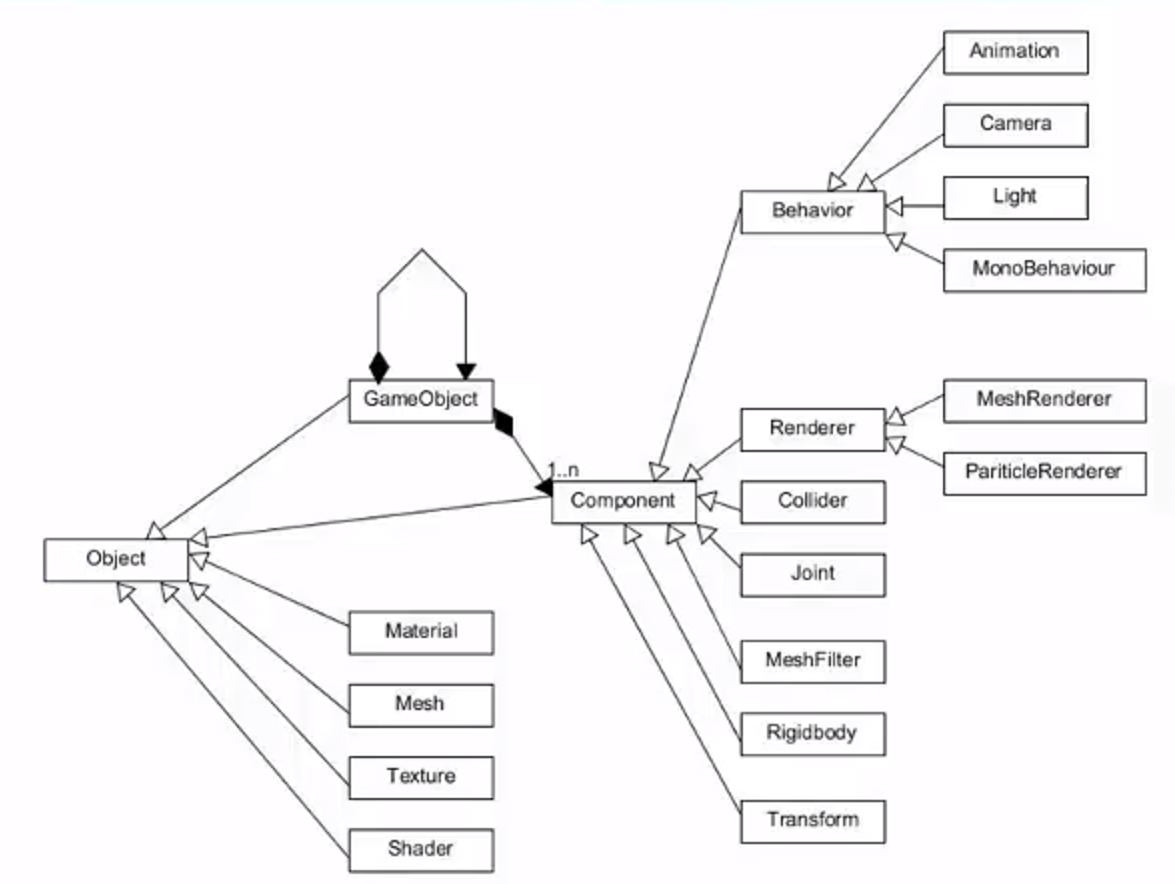
\includegraphics[scale=0.5]{class}
			\caption{Unity 类之间的关系}
		\end{figure}	
		
	\section{实体类} \verb|GameObject 类|,游戏基础对象,用于填充世界。
		\paragraph{复制}
			\verb|Instantiate(GameObject)| 或 \verb|Instantiate(GameObject, position, rotation)|
			
			\begin{itemize}
				\item \verb|GameObject |指生成克隆的\textbf{游戏对象},也可以是\textbf{Prefab 的预制品}
				\item \verb|position |克隆对象的初始位置,类型为\verb|Vector3|
				\item \verb|rotation |克隆对象的初始角度,类型为\verb|Quaternion|
			\end{itemize} 
		
		\paragraph{销毁}
			\verb|Destroy(GameObject xx)- 立即销毁 |或 \verb|Destroy(GameObject xx, Time time)- 几秒后销毁|
			
		\paragraph{可见否}
			通过设置该参数调整该实体是否可以在游戏中显示,具体设置方法为\verb|gameObject.SetActive(true) 为可以显示,false 则隐藏|
		
		\paragraph{游戏中获取或查找}
			参考:\url{https://blog.csdn.net/u010145745/article/details/39160141}
			
			\begin{enumerate}
				\item 在整个场景中寻找名为xx的游戏对象,并赋予obj 变量
					
					\verb|obj = GameObject.Find("xx");|
					
				\item 当需要获取某个\verb|gameObject| 下的组件时,使用\verb|Transform.Find.GetComponent|
					
					\verb|gameObjVar1.transform.Find("ImageItemIcon/TextMonthCardLeftDays").GetComponent<Text>().text = "xx";|
				
				\item 返回一个用tag做标识的活动的游戏物体的列表,如果没有找到则为null: 
				
					\verb|static GameObject[] FindGameObjectsWithTag (string tag);|
				
				\item 遍历场景中所有物体,获取泛型T类型物体,\verb|FindObjectsOfType(typeof(Type))|返回\verb|Type|类型的所有激活的加载的物体列表,它将返回\textit{任何资源(网格,纹理,预设,...)}\textbf{或未激活的物体}
				
					\verb|object[] gameObjects = GameObject.FindSceneObjectsOfType(typeof(Transform));|
			\end{enumerate}
	\section{Prefabs -预设体}
		prefabs基础:\url{https://www.cnblogs.com/yuyaonorthroad/p/6107320.html}
		
		动态加载Prefabs:\url{https://blog.csdn.net/linshuhe1/article/details/51355198}
		
		在进行一些功能开发的时候,我们常常将一些\textbf{能够复用的对象}制作成.\textbf{prefab的预设物体},然后将预设体存放到Resources目录之下,使用时再动态加载到场景中并进行实例化。例如:子弹、特效甚至音频等,都能制作成预设体。
		
		\subparagraph{概念} 组件的集合体, 预制物体可以实例化成游戏对象.
		\subparagraph{作用} 可以重复的创建具有相同结构的游戏对象。	
		
		\subsection{预设动态加载到场景}
			\paragraph{预设体资源加载}\verb|->|
			
				假设预设体的位置为下图所示
				\begin{figure}[H]
					\centering
					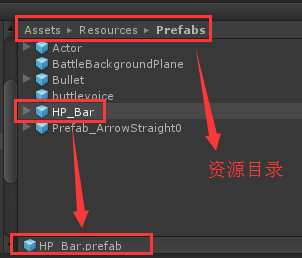
\includegraphics[scale=0.6]{Prefab-1.png}
					\caption{Prefab 资源位置}
				\end{figure}
			
				\begin{lstlisting}[xleftmargin = .079\textwidth, frame = L]
	//加载预设体资源
	GameObject hp_bar = (GameObject)Resources.Load("Prefabs/HP_Bar");				
				\end{lstlisting}
				
			通过上述操作,实现从资源目录下\textbf{载入}\verb|HP_Bar.prefab|\textbf{预设体},\textbf{用}一个\verb|GameObject|\textbf{对象来存放},此时该预设物体并未真正载入到场景中,因为还未进行实例化操作。
			
			\paragraph{预设体实例化}\verb|->|
			
				实例化使用的是\verb|MonoBehaviour.Instantiate|函数来完成的,\textbf{其实质就是从预设体资源中克隆出一个对象},它\textit{具有与预设体完全相同的属性},并且被加载到当前场景中
				
				完成以上代码之后,在当前场景中会出现一个实例化之后的对象,并且其父节点默认为当场的场景最外层,如下图所示。
					\begin{figure}[H]
						\centering
						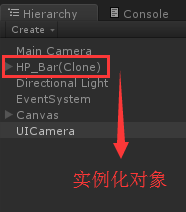
\includegraphics[scale=0.8]{Prefab-2.png}
						\caption{Prefab 实例后位置}
					\end{figure}
				
			\paragraph{实例化对象属性设置}\verb|->|
				
				完成上述步骤之后,我们已经可以在场景中看到实例化之后的对象,但是通常情况下我们\textbf{希望}我们的\textbf{对象之间层次感分明},而且这样也方便我们进行对象统一管理,而不是在Hierarchy中看到一大堆并排散乱对象,所以我们\textbf{需要为对象设置名称以及父节点等属性}。
			
				\verb|-->Notice:|常见错误:对\textbf{未初始化}的\verb|hp_bar|进行属性设置,\textbf{设置之后的属性在实例化之后无法生效}。这是\textit{因为我们最后在场景中}\textbf{显示的其实并非实例化前的资源对象},\textbf{而是一个克隆对象},\color{blue}\textit{所以假如希望设置的属性在最后显示出来的对象中生效,我们需要对实例化之后的对象进行设置}。\color{black}
			
			  正确的设置代码如下,可以看到\textbf{实例化对象}已成功挂在到\textbf{父节点Canvas}上,在层次视图效果如下图所示:
			  	\begin{lstlisting}[xleftmargin = .079\textwidth, frame = L]
	GameObject hp_bar = (GameObject)Resources.Load("Prefabs/HP_Bar");
	
	//搜索画布的方法!
	GameObject mUICanvas = GameObject.Find("Canvas");
	hp_bar = Instantiate(hp_bar);
	hp_bar.transform.parent = mUICanvas.transform;
			  	\end{lstlisting}
			  	
			  	\begin{figure}[H]
			  		\centering
			  		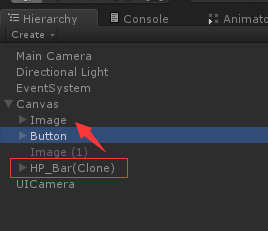
\includegraphics[scale=0.8]{Prefab-3.png}
			  		\caption{Prefab对象 设置父子关系}
			  	\end{figure}
		  	
		  		\subparagraph{简化写法}上述实例步骤与属性设置代码可以简化为
		  			\begin{lstlisting}[xleftmargin = .079\textwidth, frame = L]
	GameObject hp_bar = (GameObject)Instantiate(Resources.Load("Prefabs/HP_Bar"));
	GameObject mUICanvas = GameObject.Find("Canvas");
	hp_bar.transform.parent = mUICanvas.transform;	  				
		  			\end{lstlisting}
		  	
		  	\paragraph{预制体添加脚本}
		  		在预制体上不能直接添加脚本,首先需要将其拖入场景,然后再对其操作,这个时候可以添加脚本,添加组件等,在完成这些操作后,在Inspector 选项中选中 Apply,然后删除其在场景中的刚才拖过来的,即可。		
	\section{获取实体上的组件}
		\paragraph{调用方式}\verb|GameObject.GetComponent<Type>().xx = xx;|
			
			\begin{itemize}
				\item \verb|cube1.GetComponent<RigidBody>().mass = 20;| //设置重量
				\item \verb|cube1.GetComponent<BoxCollider>().isTrigger = true;| //\textbf{开启Trigger 穿透方式}检测
				\item \verb|cube2.GetComponent<Test>().enable = false;| //\textbf{禁用Test脚本}
			\end{itemize}
	
	\section{物理作用实体类} \verb|Rigidbody 类|,一种特殊的游戏对象,该类对象可以在物理系统的控制下来运动。
		\paragraph{AddForce()}
			此方法调用时\verb|rigidBody.AddForce(1, 0, 0);|,会施加给刚体一个瞬时力,在力的作用下,会产生一个加速度进行运动。
			
		\paragraph{AddTorque()}
			给刚体添加一个扭矩。
			
		\paragraph{Sleep()}
			使得刚体进入休眠状态,且至少休眠一帧。类似于暂停几帧的意思,这几帧不进行更新、理论位置也不进行更新。
			
		\paragraph{WakeUp()}
			使得刚体从休眠状态唤醒。
		
\chapter{世界空间相关3D基础}
	\section{Transform 类}
		\url{https://blog.csdn.net/yangmeng13930719363/article/details/51460841}
		\subsection{位置}
			\begin{itemize}
				\item \verb|transform.localPosition|:是\textbf{相对于父对象的位置},是相对坐标,既父级窗体为原点坐标
				\item \verb|transform.Position|:是\textbf{世界坐标中}的位置,可以理解为绝对坐标
			\end{itemize}
		\subsection{旋转}	
			\begin{itemize}
				\item transform.localEulerAngles 以自身坐标系为参考,而不是世界坐标系
					\begin{lstlisting}[xleftmargin = .02\textwidth]
	transform.localEulerAngles = new Vector3(x, y,z);
					\end{lstlisting}
				\item transform.rotation 以自身坐标系为参考,而不是世界坐标系
					\begin{lstlisting}[xleftmargin = .02\textwidth]
	Quaternion rotation= Quaternion.Euler(new Vector3(x, y,z));
	Transform.rotation=rotation;	
					\end{lstlisting}
				\item transform.Rotate(x,y,z)
					\begin{lstlisting}[xleftmargin = .02\textwidth]
	// 以自身坐标系为参考,而不是世界坐标系,分别以x度y度z度绕X轴、Y轴、Z轴匀速旋转
	transform.Rotate(x,y,z);
	// 以自身坐标系为参考
	transform.Rotate(轴,Space.Self);
	// 以世界坐标系为参考
	transform.Rotate(轴,Space.World);
					\end{lstlisting}
			\end{itemize}

		\subsection{缩放}
				transform.localScale(x, y, z); // 基准为1、1、1, 数为缩放因子。	
		\subsection{平移}
				transform.Translate(x, y, z); 
		\subsection{注意}
			在变化的过程中需要乘以 Time.deltaTime ,否则会出现大幅不连贯的画面。
	
	\section{Camera}
		\subsection{Clear Flags}
			清除标记。决定屏幕的哪部分将被清除。一般用户使用对台摄像机来描绘不同游戏对象的情况,有3中模式选择:
			\begin{itemize}
				\item \verb|Skybox|:天空盒。默认模式。在屏幕中的空白部分将显示当前摄像机的天空盒。如果当前摄像机没有设置天空盒,会默认用Background色。
				\item \verb|Solid Color|:纯色。选择该模式屏幕上的空白部分将显示当前摄像机的background色。
				\item \verb|Depth only|:仅深度。该模式用于游戏对象不希望被裁剪的情况。
				\item \verb|Dont Clear|:不清除。该模式不清除任何颜色或深度缓存。其结果是,每一帧渲染的结果叠加在下一帧之上。一般与自定义的shader配合使用。
			\end{itemize}
		\subsection{Culling Mask -剔除遮罩} 
			剔除遮罩,选择所要显示的\verb|layer|, \textbf{摄像机将看到勾选的层,忽略未被勾选的层。}
		
		\subsection{Projection -透视模式}
			\paragraph{透视}
				摄像机模式,\textbf{截锥体}
				
			\paragraph{正交}
				前后显示一样,不存在远小近大的样子。\textbf{长方体}
				
		\subsection{Clipping Planes -裁剪模式}
			剪裁平面。摄像机开始渲染与停止渲染之间的距离。
			
		\subsection{Viewport Rect}
			标准视图矩形。用四个数值来控制摄像机的视图将绘制在屏幕的位置和大小,使用的是屏幕坐标系,数值在0~1之间。坐标系原点在左下角。
			
		\subsection{Depth -控制渲染顺序}
			深度。\textbf{用于控制摄像机的渲染顺序},\textbf{较大}值的摄像机将\textbf{被}渲染\textit{在}\textbf{较小}值的摄像机\textbf{之上}。
			
		\subsection{Rendering Path -渲染路径}
			渲染路径。\textbf{用于指定摄像机的渲染方法}。
			
			\verb|Use Player Settings|:使用\verb|Project Settings-->Player|中的设置。
			
			\verb|Forward|:\textbf{快速渲染}。摄像机将所有游戏对象将按每种材质一个通道的方式来渲染。
			
			\verb|Defferred|: \textbf{延迟光照}
			\verb|Legacy Vertex Lit|:\textbf{顶点光照}。摄像机将对所有的游戏对象座位顶点光照对象来渲染。
			
			\verb|Legacy Deferred Lighting|:\textbf{延迟光照}。摄像机先对所有游戏对象进行一次无光照渲染,用屏幕空间大小的Buffer保存几何体的深度、法线已经高光强度,生成的Buffer将用于计算光照,同时生成一张新的光照信息Buffer。最后所有的游戏对象会被再次渲染,渲染时叠加光照信息Buffer的内容。
			
		\subsection{Target Texture -目标纹理}
			用于将摄像机视图\textbf{输出并渲染到}\textit{一张贴图}\underline{sss}。一般用于制作导航图或者画中画等效果。
			
		\subsection{HDR -高动态光照渲染}
			高动态光照渲染。用于启用摄像机的高动态范围渲染功能。
	
		\subsection{提高性问题}
			\begin{itemize}
				\item 移动摄像机的动作放在哪个系统函数中,为什么 (LateUpdate)
			\end{itemize}

	\section{3D模型}
		\subsection{Mesh}
		
		\subsection{Texture}
				
		\subsection{Material}
			尽管是近似的灰色,也同样会因为材质的不同显示出不同的效果,入灰色T恤衫和灰色不锈钢,首先是他们对光照的反应不同(漫反射、平面),其次是表面的各种属性。
			
		\subsection{骨骼动画}
	
	
	
\chapter{键盘鼠标控制}
	\section{普通按键 -keyDown(KeyCode xx)}
		\paragraph{方式一}
		
			\begin{itemize}
				\item 定义按键码:\verb|KeyCode keycode;|
				\item 判断键是否被按下:\verb|if(Input.GetKeyDown(keycode)){}|
				\item 在\verb|Inspirit -> Keycode |指定关联按键
			\end{itemize}
	
		\paragraph{方式二}
			\begin{itemize}
				\item 在\verb|Update| 中更新添加如下代码
				\item \verb|if(Input.GetKeyDown(KeyCode.UpArrow))| 
				\item \verb|KeyCode.xx |包括了键盘所有的按键,常用的AWSD 如下,鼠标同(Input.GetMouseButtonDown(0) 0左键,1右键)
					\begin{itemize}
						\item \verb|if (Input.GetKeyDown(KeyCode.S)) | 按下S键
						\item \verb|if (Input.GetKey(KeyCode.S))| 按住S键
						\item \verb|if (Input.GetKeyUp(KeyCode.W)) | 抬起S键
					\end{itemize}
			\end{itemize}
		
	\section{根据输入设备 -getAxis()}
		参数分为两类: 
		\paragraph{一、触屏类}
		 	\begin{enumerate}
			 	\item \verb|Mouse X| 鼠标沿屏幕X移动时触发 
			 	\verb|Mouse Y| 鼠标沿屏幕Y移动时触发 
			 	\verb|Mouse ScrollWheel |鼠标滚轮滚动是触发 
		 	\end{enumerate}
			
			\begin{lstlisting}
	float mouseX = Input.GetAxis("Mouse X");
	float mouseY = Input.GetAxis("Mouse Y");
	
	transform.Rotate(Vector3.Up * mouseX * rotateSpeed); // 根据具体需求进行操作
			\end{lstlisting}
		
		\paragraph{二、键盘类}
		 	\begin{enumerate}
		 		\item Vertical 键盘按上或下键时触发 
		 		\item Horizontal 键盘按左或右键时触发
		 	\end{enumerate}
		 	
		 	\begin{lstlisting}
	float horizontal = Input.GetAxis("Horizontal");
	float vertical = Input.GetAxis("Vertical");
	
	Vector3 desPos = (transform.forward * vertical  + transform.right * horizontal) * Time.deltaTime * moveSpeed;
	
	_rigidBody.position += desPos;
		 	\end{lstlisting}
		\textbf{返回值}是一个数,正负代表方向
		
		\paragraph{三、继承IPointerDrag等}
			
\chapter{时间}
 	\section{Time 类}
 		该类是 U3D 在游戏中获取时间信息的接口类。常用变量如下:
 		
 		\begin{table}[H]
 			\centering
 			\caption{时间变量对照表}
 			\begin{tabular}{m{4cm}|m{10cm}}
 				\toprule
 					变量名 & 意义\\
 				\midrule
 					time & 单位为秒 \\
 					\verb|deltaTime|     & 从上一帧到当前帧消耗的时间 \\
 					fixedTime     & 最近FixedUpdate 的时间,从游戏开始计算 \\
 					\verb|fixedDeltaTime|     & 物理引擎和FixedUpdate 的更新时间间隔 \\
 					timeSceneLevelLoad     & 从当前Scene 开始到目前为止的时间 \\
 					realTimeSinceStartup     & 程序已经运行的时间 \\
 					\verb|frameCount|     & 已经渲染的帧的总数 \\
 				\bottomrule 
 			\end{tabular}
 		\end{table}
 		 		

\chapter{数学}
	\section{Random 类}
		随机数类
		
	\section{Mathf 类}
		数学类
	
	\section{坐标系}
		左右手坐标系:\url{http://www.cnblogs.com/mythou/p/3327046.html}
	
	\section{向量计算}
	
	
	\section{矩阵计算}
	
	
	
\chapter{光照}
	\section{光照}
		
	\section{烘培}
		\paragraph{简介}
			只有静态场景才能完成烘培(Bake)操作,其目的是在游戏编译阶段完成光照和阴影计算,然后以贴图的形式保存在资源中,以这种手段避免在游戏运行中计算光照而带来的CPU和GPU损耗。
			
			\begin{itemize}
				\item \textbf{如果不烘培}:游戏运行时,这些阴影和反光是由CPU和GPU计算出来的。
				\item \textbf{如果烘焙}:游戏运行时,直接加载在编译阶段完成的光照和阴影贴图,这样就不用再进行计算,节约资源。
			\end{itemize}
		
		\paragraph{流程}
	
	
\chapter{寻路}
	\section{简介}
		NPC 完成自动寻路的功能。
		
	\section{流程}
		\begin{itemize}
			\item 将静态场景调至(Navigation Static)
			\item 烘焙
			\item 添加 \verb|Navigation Mesh Agent| 寻路组件
			\item 在脚本中设置组件的目标地址,添加目标
		\end{itemize}
	
\chapter{UGUI}
	在脚本中使用时记得加上\verb|using UnityEngine.UI |
	
	\url{https://blog.csdn.net/wangmeiqiang/article/category/6364468}
	
	\section{Spirit}
		在UI系统中,\textbf{所有的图片的显示}\underline{都必须}\textit{通过Spirit。}
		
		如果建立工程时选择的是2D工程,那么导入的所有图片会自动设置为\textit{Spirit。}
		
		如果建立工程时选择的是3D工程,那么导入的所有图片需要手动的设置为\textit{Spirit。}\verb|Inspector -> Texture Type -> Spirit(2D and UI)|,最后点击Apply 保存更改。
	
	\section{Canvas}
		Canvas画布\textbf{是承载所有UI元素的区域}。\verb|Canvas|实际上\textbf{是一个游戏对象}上\textbf{绑定了Canvas组件}。
		
		\textbf{所有的UI元素}都\textbf{必须是Canvas的子对象}。如果场景中没有画布,那么我们创建任何一个UI元素,都会自动创建画布,并且将新元素置于其下。
		
		在Canvas的\verb|Render Mode|中有三个选择:
			\begin{enumerate}[itemindent = 1em]
				\item Screen Space - Overlay 屏幕最上层,主要是2D效果。
				\item Screen Space - Camera 绑定摄像机,可以实现3D效果。
				\item World Space 世界空间,让UI变成场景中的一个物体。
			\end{enumerate}
	
		\subsection{Screen Space-Overlay -覆盖模式}
			Screen Space-Overlay(屏幕控件-覆盖模式)的\textbf{画布会填满整个屏幕空间},并将画布下面的所有的UI元素置于屏幕的最上层,或者说\textbf{画布的画面永远“覆盖”其他普通的3D画面},\textit{如果屏幕尺寸被改变,画布将自动改变尺寸来匹配屏幕}
			
			Screen Space-Overlay模式的画布有Pixel Perfect和Sort Layer两个参数:
			\begin{enumerate}[itemindent = 1em]
				\item \verb|Pixel Perfect|:只有\verb|RenderMode|为Screen类型时才有的选项。使UI元素像素对应,效果就是\textbf{边缘清晰不模糊}。
				\item \verb|Sort Layer|: \verb|Sort Layer|是UGUI专用的设置,用来指示\textbf{画布的深度}。
			\end{enumerate}
		
		\subsection{Screen Space-Camera -摄像机模式}
			与Screen Space-Overlay模式类似,画布也是\textbf{填满整个屏幕空间},如果屏幕尺寸改变,\textbf{画布也会自动改变尺寸来匹配屏幕}。
			
			不同的是,在该模式下,\textbf{画布会被放置到摄影机前方}。在这种渲染模式下,\textbf{画布看起来 绘制在一个与摄影机固定距离的平面上}。\textit{所有的UI元素都由该摄影机渲染,因此摄影机的设置会影响到UI画面}。在此模式下,UI元素是由\verb|perspective|也就是视角设定的,视角广度由\verb|Filed of View|设置。
			
			\textbf{这种模式可以用来实现在UI上显示3D模型的需求},比如很多MMO游戏中的查看人物装备的界面,可能屏幕的左侧有一个运动的3D人物,左侧是一些UI元素。通过设置Screen Space-Camera模式就可以实现上述的需求,效果如下图所示:
				\begin{figure}[H]
					\centering
					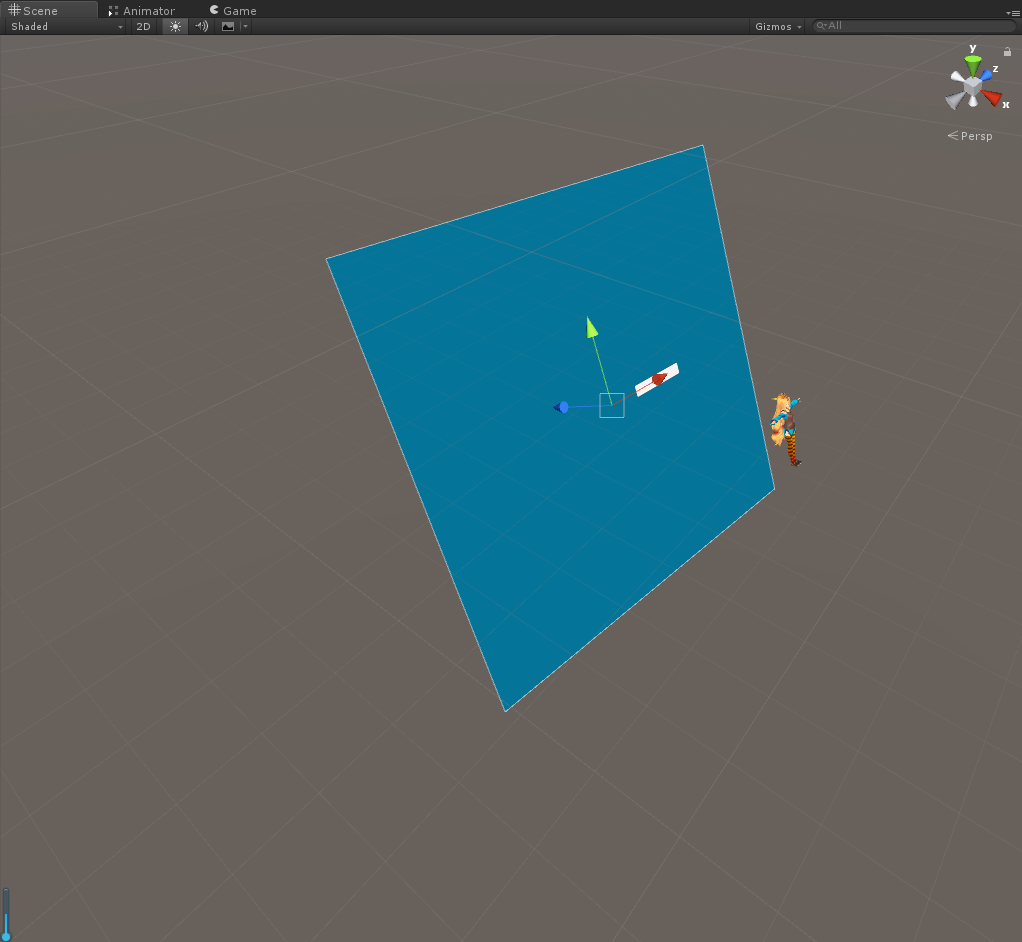
\includegraphics[scale=0.3]{Canva-1.png}
					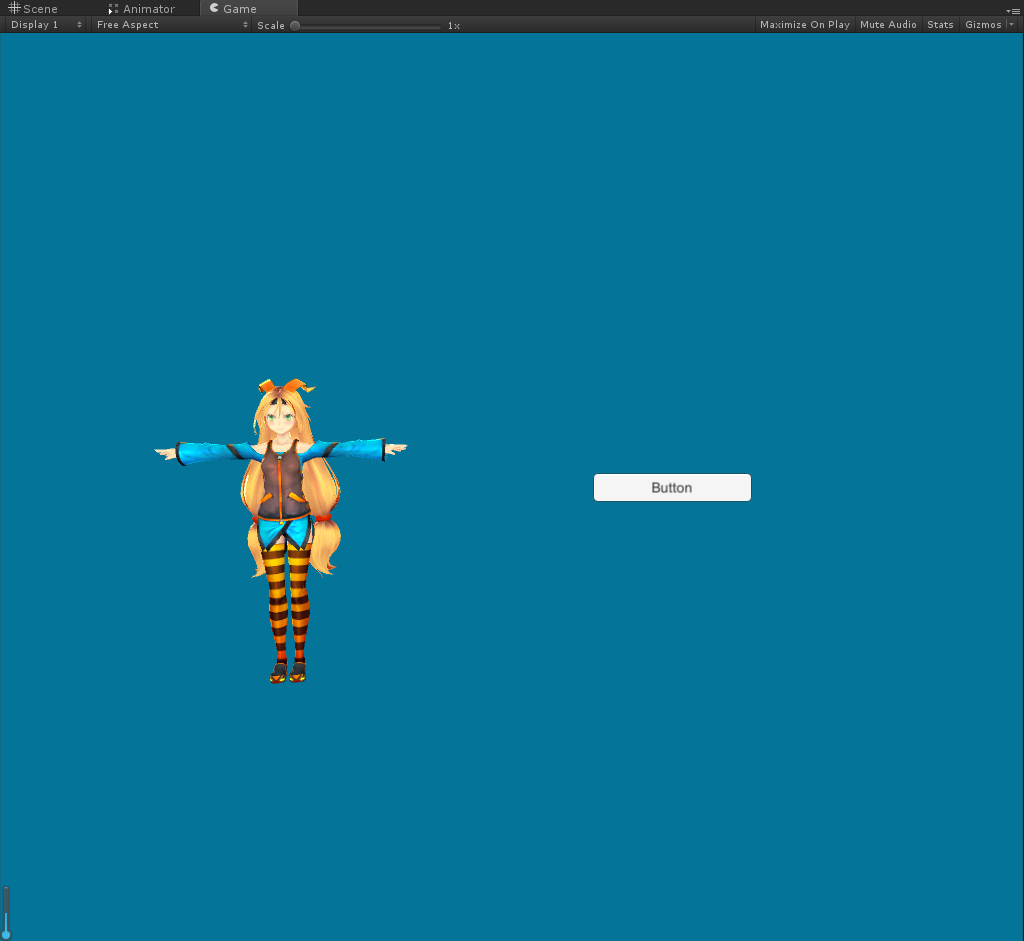
\includegraphics[scale=0.3]{Canvas.png}
					\caption{摄像机模式-画布}
				\end{figure}
			
			它比Screen Space-Overlay模式的画布多了下面几个参数:
				\begin{enumerate}[itemindent = 1em]
					\item \verb|Render Camera|:渲染摄像机
					\item \verb|Plane Distance|:\textbf{画布距离摄像机的距离}
					\item \verb|Sorting Layer|: Sorting Layer是UGUI专用的设置,\textbf{用来指示画布的深度}。可以通过点击该栏的选项,在下拉菜单中点击“Add Sorting Layer”按钮进入标签和层的设置界面,或者点击导航菜单->edit->Project Settings->Tags and Layers进入该页面。
					\item \verb|Order in Layer|:\textbf{在相同的Sort Layer下的画布显示先后顺序。}数字越高,显示的优先级也就越高。
				\end{enumerate}
				
				depth 参考世界空间相关一章,camera Depth.
			
		\subsection{World Space -世界空间模式}
			World Space即世界空间模式。在此模式下,\textbf{画布被视为与场景中其他普通游戏对象性质相同的类似于一张面片(Plane)的游戏物体}。
			
			画布的尺寸可以\textbf{通过RectTransform设置},所有的UI元素可能位于普通3D物体的前面或者后面显示。\textbf{当UI为场景的一部分时,可以使用这个模式}。
			
				\begin{figure}[H]
					\centering
					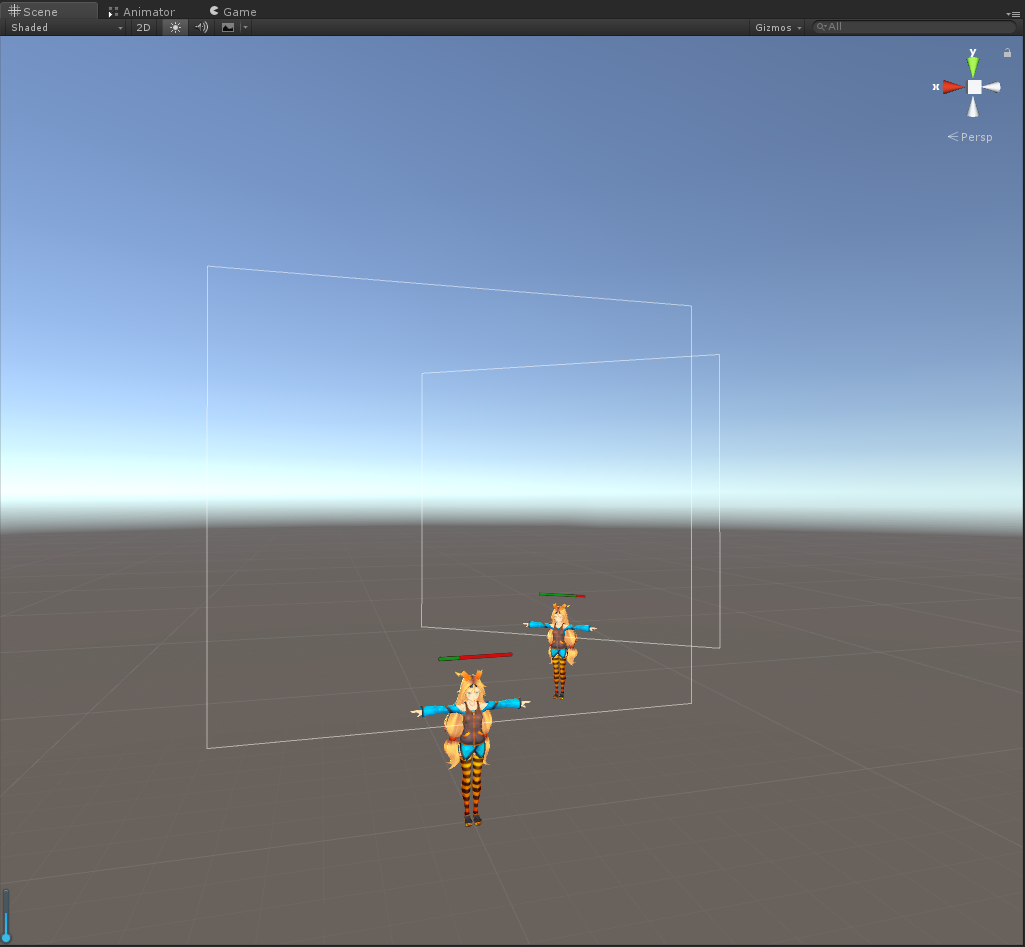
\includegraphics[scale=0.3]{Canvas-2.png}
					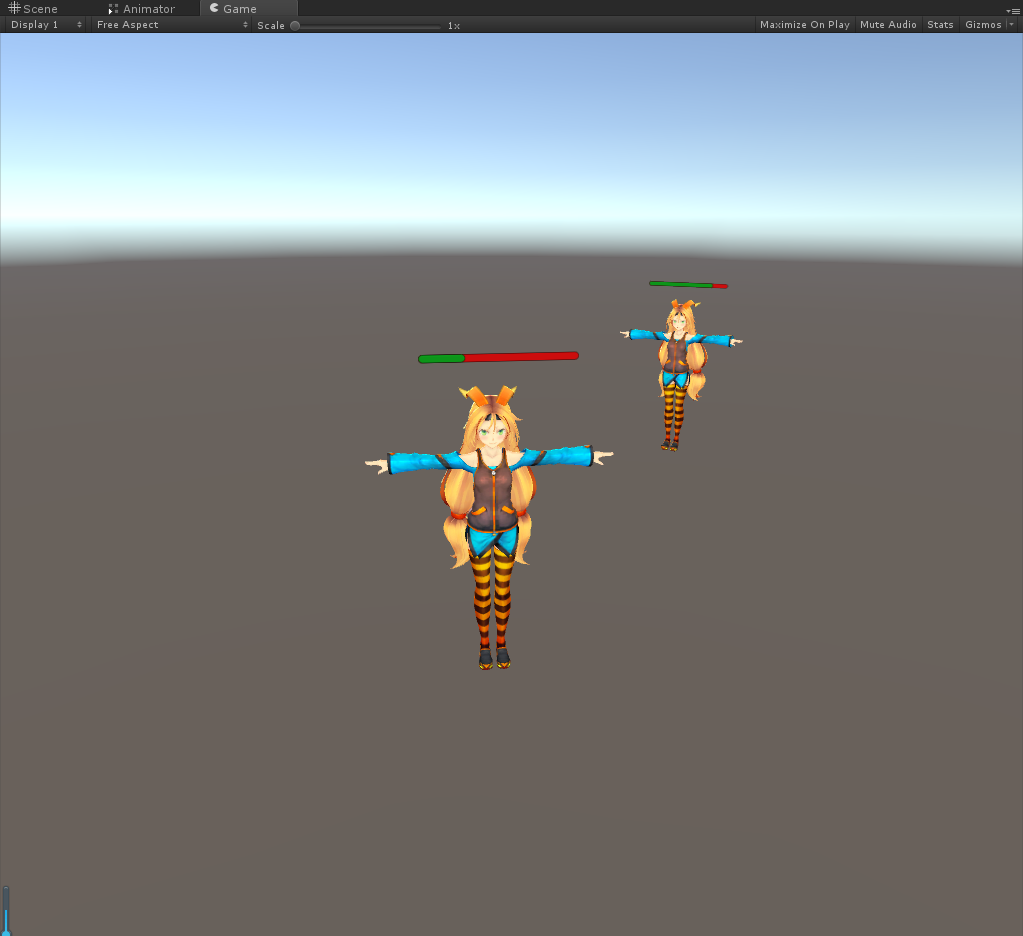
\includegraphics[scale=0.3]{Canvas-3.png}
					\caption{世界空间 模式- 画布}
				\end{figure}
			
		
		\subsection{使用总结}
			\begin{table}[H]
				\centering
				\caption{渲染模式使用场景说明}
				\begin{tabular}{p{5cm}<{\centering}|c|c|c|p{4cm}<{\centering}}
					\toprule
						渲染模式 & 画布匹配屏幕?& 摄像机? & 像素对应 & 适应\\
					\midrule
						覆盖-overlay模式 & 是	& 不需要	& 可选 & 2D \\
						摄像机-camera模式 & 是	& 需要	 & 可选 & 2D+3D\\
						世界空间-world模式 & 否	& 需要	 & 不可选 & 3D\\
					\bottomrule
				\end{tabular}
			\end{table}
		
		\subsection{Canvas Scalar}
			\textbf{“The Canvas Scaler component is used for controlling the overall scale and pixel density of UI elements in the Canvas. This scaling affects everything under the Canvas, including font sizes and image borders.”}

			用于画布上UI元素的整体缩放比例和像素密度。该缩放比例会影响画布中的所有东西,包括字体大小和图像边界。
			
			为了适应不同的分辨率,我们可能会\textbf{允许适当的UI整体性的缩放,外加一些尽可能少的布局微调}。这样就能达到一个比较理想的效果。Unity中 Canvas Scale就是负责该功能的组件。
			 
			Canvas Scaler的ui scale mode有三种值(constan pixel size、scale with screen size和constant physical size)
			
			\begin{table}[H]
				\centering
				\caption{简介}
				\begin{tabular}{p{4.5cm}<{\centering}|p{11.5cm}<{\centering}}
					\hline
						UI缩放模式 &  决定画布中的UI元素如何缩放\\
					\hline
						Constant Pixel Size & 不管屏幕尺寸如何变化,UI元素保持相同的像素大小\\
						Scale With Screen Size & 屏幕越大,UI元素也越大\\
						Constant Physical Size & 不论屏幕大小和分辨率如何变化,UI元素保持相同的物理尺寸\\
					\hline
				\end{tabular}
			\end{table}
			
			\begin{itemize}
				\item \textbf{Constant Pixel Size}这个模式一般用于需要整体缩放画布的对象(通过Scale Factor)
					\begin{enumerate}
						\item Scale Factor: 画布的缩放比例。默认况下为1,表示正常大小。
						\item Reference Pixels Per Unit: 每单位代表的像素量
					\end{enumerate}
				\item \textbf{Constant Physical Size} 和前面这个类似也可以缩放(通过RectTransform)
					
				\item \textbf{Scale With Screen Size} 这个模式比较常用是我们开发自适应一般用的模式
					\begin{enumerate}
						\item Reference Resolution(参考分辨率) :参照这个UI布局所依据的分辨率,如果屏幕分辨率更大,那么UI会变大,如果屏幕分辨率更小,那么UI会变小。
						\item Screen Match Mode(屏幕匹配模式) :Match Width or Height、Expand、Shrink
						\item Reference Pixels Per Unit 每单位的参考像素
					\end{enumerate}
			\end{itemize}

			\url{https://blog.csdn.net/gz_huangzl/article/details/52484611}
			
			
			\begin{table}[H]
				\centering
				\caption{Scale With Screen Size}
				\begin{tabular}{p{4.5cm}<{\centering}|p{11.5cm}<{\centering}}
					\hline
						属性 &  功能\\
					\hline
						参考分辨率 &  再设计UI布局时设置的分辨率,如果屏幕分辨率更大,UI元素也会放大,反之亦然   \\
						屏幕匹配模式 &   当前分辨率下的宽高比不适合参考分辨率时使用的一种用于缩放画布的模式 \\
						匹配宽度或高度 &  用宽度或者高度又或者两者之间做参考来缩放画布 \\
						扩展 & 水平或垂直扩展画布,所以画布的尺寸不会比参考分辨率小\\
						收缩 & 水平或垂直裁剪画布,所以画布的尺寸不会比参考分辨率大\\
						匹配 & 决定缩放时,使用宽度/高度/两者之间用作参考\\
						参考的每单位像素 & 如果一个sprite 有“每单位像素数” 这个设置,那么spirit 中的一个像素会覆盖UI中的一个单元\\						 
					\hline
				\end{tabular}
			\end{table}
		\subsection{Layer}
		
		
	\section{RectTransform}
		\url{https://blog.csdn.net/jk823394954/article/details/53861539}
	
		\url{https://blog.csdn.net/rickshaozhiheng/article/details/51569073}
		
		\url{https://blog.csdn.net/serenahaven/article/details/78826851}
		
		\url{https://www.jianshu.com/p/dbefa746e50d}
		
		核心看:\url{https://blog.csdn.net/Happy_zailing/article/details/78835482}
		
		\url{http://lib.csdn.net/article/unity3d/36875}
		
		RectTransform继承自Transform, 又增加锚点、中心轴点等信息,\textbf{主要提供一个矩形的位置、尺寸、锚点和中心信息以及操作这些属性的方法},\textit{同时提供多种基于父级RectTransform的缩放形式}。
		
		\subsection{Pivot(中心)}
			Pivot用来指示一个\verb|RectTransform|(或者说是矩形)的中(重)心点。	
	
		\subsection{锚点- 自适应屏幕}
			\url{http://www.bubuko.com/infodetail-2384845.html}
			
			
			锚点(四个)由\verb|两个Vector2|的向量确定,这两个向量确定两个点,归一化坐标分别是\verb|Min|和\verb|Max|,\textbf{再由这两个点确定一个矩形},\textbf{这个矩形的四个顶点就是锚点}。
			
			在\verb|Hierarchy|下新建一个Image,查看其\verb|Inspector|。
			
			\begin{figure}[H]
				\centering
				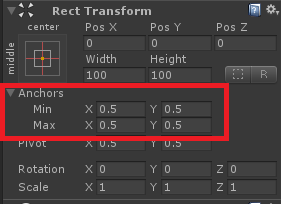
\includegraphics[scale=1.2]{Anchor.png}
				\caption{Anchor 属性}
			\end{figure}
			
			在Min的x、y值分别小于Max的x、y值时,
			\verb|Min |确定矩形\textbf{左下角}的归一化坐标,\verb|Max |确定矩形\verb|右上角|的归一化坐标。
			
			刚创建的Image,其\verb|Anchor的默认值 |为\verb|Min(0.5,0.5)|和\verb|Max(0.5,0.5)|。也就是说,\verb|Min和Max|重合了,四个锚点合并成一点。锚点在Scene中的表示如下:
			
			\begin{figure}[H]
				\centering
				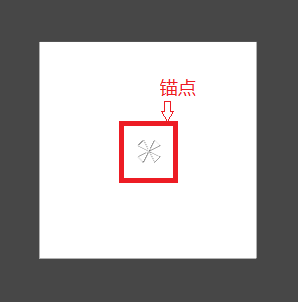
\includegraphics[scale=0.7]{anchorFirst.png}
				\caption{锚点初始位置}
			\end{figure}
		
			将Min和Max的值分别改为\verb|(0.4,0.4)|和\verb|(0.5,0.5)|。可以看见四个锚点已经分开了。
			
			\begin{figure}[H]
				\centering
				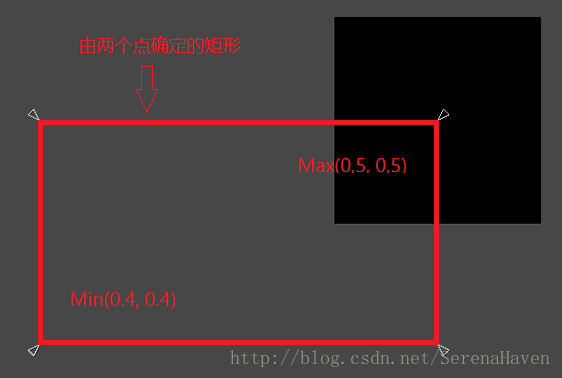
\includegraphics[scale=0.5]{anchorChange.png}
				\caption{min Max位置、确定矩形}
			\end{figure}
			
			
			\subparagraph{需要注意} 在不同的Anchor设置下,控制该RectTransform的变量是不同的。
			
			比如设置成全部居中(默认)时,属性里包含熟悉的用来描述位置的\verb|PosX、PosY和PosZ|,以及用来描述尺寸的\verb|Width和Height|;
			
			切换成全部拉伸时,属性就变成了\verb|Left、Top、Right、Bottom|和\verb|PosZ|,\textbf{前四个属性}用来描述该RectTransform\textbf{分别离父级各边的距离},PosZ用来描述该RectTransform在世界空间的Z坐标
			
			\paragraph{锚点类型}
				\begin{itemize}
					\item 位置类型\verb| 左上角、中心等|
					\item 拉伸类型\verb| 纵向拉伸适配、横向、整体|
				\end{itemize}
		
				\subparagraph{锚点在一块的时候}
					\begin{itemize}[itemindent = 2em]
						\item Anchor 是打在父级窗体上的
						\item Anchor 的位置在父级窗体上的标记方式是按照百分比记录的,单位(百分比)
						\item Anchor 的\verb|Min(RectTransform.anchorMin)  Max(RectTransform.anchorMax)|的信息保持一致
						\item 子物件的 坐标系 为纵向Y,横向X, 并且以\verb|Anchor| 为原点, 自身坐标用中心轴点\verb|Pivot| 表示						
						\item 子物件的 Pivot 与 Anchor  位置始终保持不变,单位(像素)
					\end{itemize}
				
				\subparagraph{锚点单向(横或者纵)分开的时候}
					\begin{itemize}[itemindent = 2em]
						\item 分开的部分(拉伸方向)与父级窗体保持一致变化,单位(百分比)
						\item 与相对方向则绝对保持,单位(像素)
					\end{itemize}
				
				\subparagraph{锚点双向分开的时候}
					\begin{itemize}[itemindent = 2em]
						\item 双向 都与 父级窗体 保持一致的变化,单位(百分比)
						\item 上-top、下-bottom、左、右边距绝对保持,单位(像素)
					\end{itemize}
		
			\paragraph{anchorMax、anchorMin}
				\verb|anchorMin.x|表示锚点在\verb|x|轴的起始点位置,\verb|anchorMax.x|表示锚点在x轴的终点位置,取值\verb|0~1|,表示\textbf{百分比值},该值乘以父窗口的\verb|width|值就是实际锚点相对于父窗口x轴的位置。y轴与x轴同理。
		
					\begin{figure}[H]
						\centering
						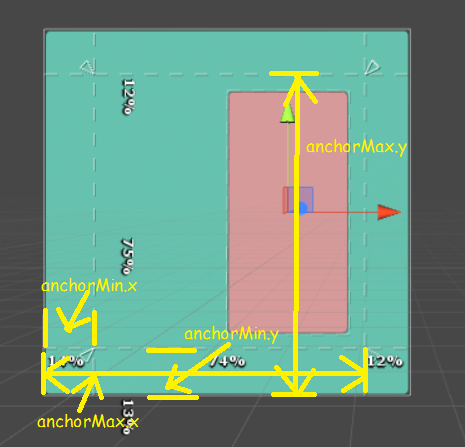
\includegraphics[scale=0.8]{Anchors-3.png}
						\caption{Anchor.Min 与 Anchor.Max}
					\end{figure}
		
				这个值确定了锚点相对于父窗口的位置,是\textbf{真正决定锚点位置的值}
				
			\paragraph{offsetMax 和 offsetMin 属性}
				\subparagraph{锚点 分开时}
					在锚点分开的状态下: 锚点其实是四个钉子,分为左上,左下,右下及右上四个,每个空间在UI模型中都是一个矩形,也有左上,左下,右下及右上四个顶点,那么锚点的每个钉子可以关联一个点,即左上————左上;左下————左下;右下————右下;右上————右上。这样进行绑定。
					
					\verb|offsetMax |是RectTransform\textbf{右上角相对于右上Anchor的距离};
			
					\verb|offsetMin |是RectTransform\textbf{左下角相对于左下Anchor的距离}。
			
					\verb|offset |可以认为是以像素为单位。
					
					\begin{figure}[H]
						\centering
						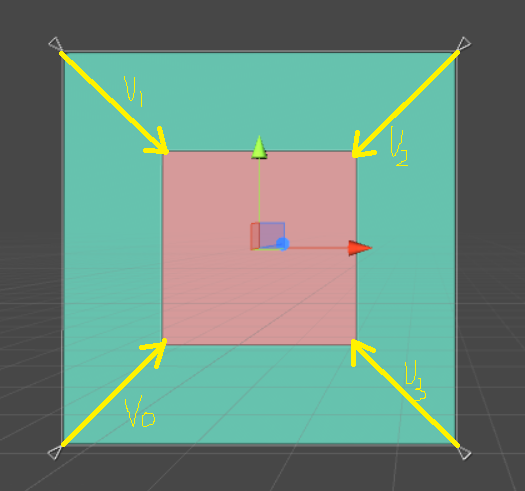
\includegraphics[scale=0.7]{Anchors-1.png}
						\caption{锚点在一起时  Offset 求取向量示例}
						\label{锚点分开时 Offset 求取向量示例}
					\end{figure}
			
				\subparagraph{锚点 在一处时}
					锚点offset 计算如下:
					
					\begin{figure}[H]
						\centering
						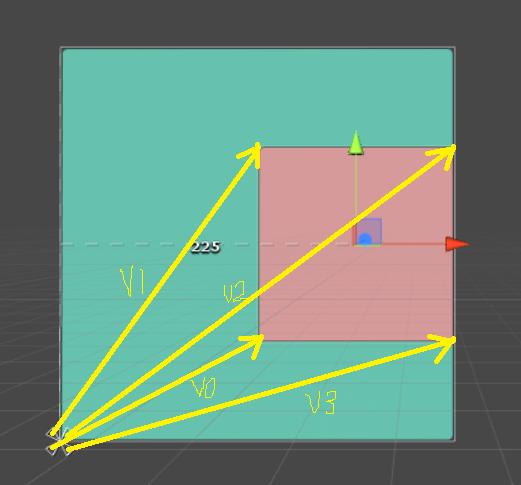
\includegraphics[scale=0.7]{Anchors-2.png}
						\caption{锚点分开时  Offset 求取向量示例}
					\end{figure}
			
				\subparagraph{求取}
					首先计算锚点的每个钉子到其对应的顶点矢量值,分别记作\verb|v0|,\verb|v1|,\verb|v2|,\verb|v3|, 入上图。
					
					然后比较四个向量的\verb|x|值,将\verb|x|的最大值赋给\verb|offsetMax.x|,将\verb|x|的最小值赋给\verb|offsetMin.x|;\verb|y|的值同理。
			
			\paragraph{anchoredPosition}
				\subparagraph{锚点 在一处时}
					anchorPosition 就是 \textbf{从锚点}到本物体的\textbf{轴心}(Pivot)的\textbf{向量值}.
				
				\subparagraph{锚点 分开时}
						
		\subsection{sizeDelta}
		
			\verb|sizeDelta|是\verb|offsetMax-offsetMin|的结果。在\textit{锚点全部重合的情况下},它的值就是面板上的\verb|(Width,Height)|。
			
			\textit{在锚点完全不重合}的情况下,它是相对于父矩形的尺寸。
			
			一个常见的错误是,当RectTransform的锚点\textbf{并非全部重合时},使用sizeDelta作为这个RectTransform的尺寸。此时拿到的结果一般来说并非预期的结果。
			
		\subsection{RectTransform.rect}	
			RectTransform.rect 的各值如图所示。
			
			\begin{figure}[H]
				\centering
				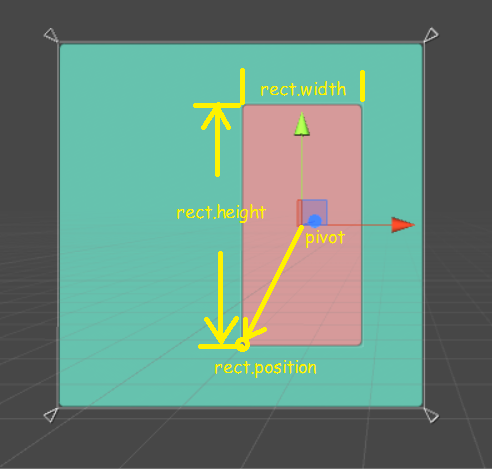
\includegraphics[scale=0.8]{RectTransform-rect.png}
				\caption{RectTransform rect 属性}
			\end{figure}	
		
		\subsection{示例}
			\begin{lstlisting}
	GameObject webText = new GameObject("webText");
	webText.AddComponent<UnityEngine.UI.Text>();
	webText.GetComponent<UnityEngine.UI.Text>().text = "";
	webText.GetComponent<RectTransform>().anchorMin = new Vector2(0, 0);
	webText.GetComponent<RectTransform>().anchorMax = new Vector2(1, 1);
	webText.GetComponent<RectTransform>().sizeDelta = new Vector2(0, 0);
	webText.GetComponent<RectTransform>().anchoredPosition = new Vector2(0, 0);
	webText.transform.localPosition = new Vector3(0,0,0);
	webText.transform.SetParent(webObj.transform, false);
			\end{lstlisting}
			
		\subsection{FramDebug}
			查看渲染的先后顺序
			
			\verb|windows->FrameDebug |	
	\section{按钮}
		\subsection{RayCast Target-点击事件的获取原理}
			参考文献:\url{https://blog.csdn.net/liujunjie612/article/details/55097789}
			
			UGUI会遍历屏幕中所有RaycastTarget是true的UI,接着就会发射线,并且排序找到玩家最先触发的那个UI,在抛出事件给逻辑层去响应。
			
			团队多人在开发游戏界面,很多时候都是复制黏贴,比如上一个图片是\textbf{需要响应}RaycastTarget,然后ctrl+d以后复制出来的也就带了这个属性,很可能新复制出来的图片是\textbf{不需要响应的},开发人员\textbf{又没有取消勾选掉},\textit{这就出问题了}。
			
			所以RaycastTarget如果被勾选的过多的话, 效率必然会低。
		\subsection{原始Button}
			
		\subsection{Image等 -添加button 组件}
			\begin{itemize}
				\item \verb|create -> UI -> Image|
				\item \verb|Inspirit -> Add Component -> button|
			\end{itemize}	
		
		\subsection{添加事件处理脚本}
			\begin{itemize}
				\item 书写脚本并添加到Button gameObject 上
				\item 如果是Button 组件的话直接在button 组件上添加,如果是Image 则添加button 组件后再添加
				\item  添加脚本对象到\verb|onClick() |部分:\verb|+ -> gameObject 拖进来  -> 选择脚本中的具体函数|
			\end{itemize}
		
	\section{文本- Text}
		\subsection{添加文字阴影 -shadow 组件}
			\verb|addComponent -> shadow|
			
		\subsection{添加文子边框 -outline 组件}
			\verb|addComponent -> outline|
			
	\section{图片- ImageView}
		
	\section{选中标记- Toggle}
		\paragraph{Toggle 基本}
		
		\paragraph{Toggle Group}
			\subparagraph{选项栏设定}
				将panel  拖入 toggle 中的\verb|value changed|部分
				
			\subparagraph{预设}
				确定默认打开哪个panel,然后将其\verb|IsOn| 勾选,其余取消勾选	
				
	\section{滚动区域、滚动条}
	
	
	\section{其他工具条}
	
	\section{布局- Layout}
		\begin{itemize}
			\item 具体页面下创建空物体 \verb| GameObject|
			\item 其次在\verb|GameObject 下|添加组件 \verb|-> grid layout group|
			\item 最后在这个\verb|GameObject |下创建出各种Image 组件,然后这些组件将会以\verb|grid layout| 的布局进行自动调整
		\end{itemize}
	
		\subsection{grid layout group}
			\begin{itemize}
				\item  调整\verb|cell size| 进行调整子物件的大小
				\item  \verb|cell size| 的改变只影响子组件的第一层,既最下面一层
			\end{itemize}
		
		\subsection{horizontal layout group}
		
		\subsection{vertical layout group}

	\section{提高性问题}
		\begin{itemize}
			\item 为什么UI摄像机和场景摄像机能协同工作
			\item 怎么防止UI控件被点穿(如何过滤掉点击事件)
			\item UI功能模块之间相互通信有什么好看法。(或者问成Broadcast和sendMes的看法)
			\item 屏幕适配有什么好主意
		\end{itemize}
		
		
		
\chapter{物理}
	\section{具体相关类}
		\subsection{Rigidbody}
			刚体,套上这个组件的\textbf{物体会受到物理作用里的影响}(包括重力,推力,作用力等一切物理力),\textit{如果没有这个组件物体也会静止不动}.
			
			\textbf{但必须有碰撞检测组件才能保证物体不被穿过}。值得注意的一点是,Is Kinematic被勾选上表示物体不接受物理力的作用,只能通过transform的设置改变位置。
		
		\subsection{Collider}
			碰撞检测器,就是\textbf{检测一切范围内的触碰事件},注意也就是说rigidbody的物理碰撞需要collider来检测才能发生,也就是物体的运动。
		
			在\textbf{所有Collider上}有一个\verb|Is Trigger| 的\verb|bool|型参数。当发生碰撞反应的时候,\textbf{会先检查此属性}。
				
			\verb|Is Trigger| 好比是一个物理功能的开关, \textbf{是要}“物理功能”\textbf{还是要}“OnTrigger脚本”。
			\begin{itemize}
				\item 碰撞器有碰撞的效果,\verb|IsTrigger=false|,可以调用\verb|OnCollisionEnter/Stay/Exit|函数
				\item 触发器没有碰撞效果,\verb|IsTrigger=true|,可以调用\verb|OnTriggerEnter/Stay/Exit|函数
			\end{itemize}
	
	\section{碰撞器、触发器}
		在Unity中参与碰撞的物体分2大块:1.发起碰撞的物体。2.接收碰撞的物体。
		
		\paragraph{发起碰撞的物体}
			Rigodbody , CharacterController(其中的RigidBody) 
		
		\paragraph{接收碰撞的物体}
			所有的Collider
			
		工作的原理为:发生碰撞的物体中必须要有“\textbf{发起碰撞}”的物体。否则,碰撞不响应。
		
		判断碰撞就是需要计算力,无论是阻力也好,动力也好,\textbf{如果此时物体有刚体组件,那么物体就会在力的作用下运动}。\textit{如果这个物体没有刚体,那么碰撞产生的力就没有任何意义了},那计算碰撞也就没有任何意义了。
		
		\textbf{所以,如果两个碰撞体都没有刚体组件,那么这两个物体即使相互发生了碰撞,那么也不会有碰撞事件的}。

		\paragraph{物体发生碰撞的必要条件}
			两个物体\textbf{都必须}带有\verb|碰撞器(Collider)|,\textbf{其中一个}\textbf{还必须}带有\verb|Rigidbody|。
		
		\paragraph{CharacterController和Rigidbody的区别}
			\begin{itemize}
				\item CharacterController自带胶囊碰撞器,里面包含有刚体的属性
				\item Rigidbody就是刚体,使物体带有刚体的特征
			\end{itemize}
	
		\paragraph{碰撞过程}
			\begin{enumerate}
				\item OnCollisionEnter
				\item OnCollisionStay
				\item OnCollisionExit
			\end{enumerate}
		
		\paragraph{施加力的方式}都在rigidbody 系列函数中。
			\begin{itemize}
				\item rigidbody.AddForce()
				\item rigidbody.AddForceAtPosition()
			\end{itemize}	
			
	\section{物理材质}
	
	\section{射线}
		\paragraph{射线 Ray}
			\verb|Ray ray = Camera.main.ScreenPointToRay(Input.mousePosition);|
			
			可以从摄像机发出一条射线到MousePosition。
			
			
		\paragraph{射线检测 Physics.Raycast()}
			\begin{itemize}[itemindent = 1em]
				\item \fbox{static bool Raycast(Ray ray, RaycastHit hitInfo, float distance, int layerMask);}
				\item \fbox{Raycast(Ray ray, float distance, int layerMask);}
				\item \fbox{Raycast(Vector3 origin, Vector3 direction, float distance, int layerMask);}
				\item \fbox{Raycast(Vector3 origin, Vector3 direction, RaycastHit , float distance ,int layerMask );}
			\end{itemize}
			
			\verb|Ray ray|是射线;\verb|RaycastHit hitInfo|是碰撞信息;\verb|float distance|是碰撞距离;\verb|int layerMask|是碰撞的层.
			
			\textbf{RaycastHit} 是输出参数,所以需要先声明一个作为参数提供。其具体包括如下信息:
			\begin{itemize}[itemindent = 1em]
				\item \verb|point| 射线碰到碰撞器的碰撞点,在世界空间中
				\item \verb|normal| 射线所碰到的表面的法线
				\item \verb|distance| 从光线的原点到碰撞点的距离
				\item \verb|collider| 碰撞到的碰撞器
				\item \verb|transform| 碰到的物体的位置信息
			\end{itemize}
			
			\verb|Physics.Raycast(ray, out hit, 100f, targetMask)|
			
			一条\textbf{射线},\textbf{射线的范围}是100米,只和\textbf{target层}发生碰撞,碰撞后得到碰撞体的信息,并返回一个布尔值。
	
	\section{关节}
		
\chapter{动画}
	\section{游戏动画有哪几种,以及其原理}
		\subsection{关节动画}
			把角色分成若干独立部分,一个部分对应一个网格模型,部分的动画连接成一个整体的动画,角色比较灵活,Quake2中使用这种动画。 
			
		\subsection{单一网格模型动画}
			由一个完整的网格模型构成,在动画序列的关键帧里记录各个顶点的原位置及其改变量,然后插值运算实现动画效果,角色动画较真实。   
			
		\subsection{骨骼动画}
			广泛应用的动画方式,集成了以上两个方式的优点,骨骼按角色特点组成一定的层次结构,有关节相连,可做相对运动,皮肤作为单一网格蒙在骨骼之外,决定角色的外观,皮肤网格每一个顶点都会受到骨骼的影响,从而实现完美的动画。
	
	\section{Avatar}
		\dirtree{%
			.1 创建Avatar .
			.2 配置Avatar . 
			.3 肌肉设定 .
			.4 动画重定位 .
			.5 反向动力学 .
		}	
	
		\url{https://www.cnblogs.com/rainmj/p/5451847.html}
		
	\section{Animation}
		\dirtree{%
			.1 .
			.2 在要动态显示的物体的父节点上创建\textbf{Animation}-(在Animation 窗口创建、在Parameter 下添加需要改变状态的组件,在关键帧修改其状态) .
			.3 编辑Animation .
			.4 在脚本中获取该父亲节点上的Animator 组件 .
			.5 播放动画 .
		}
		
	
			
	\section{Animator}

		\paragraph{打开动画状态机界面}	
				\begin{enumerate}
					\item 右键点击“Assets”栏空白处,同样可以打开菜单栏进行创建:Create->Animater Controller
					\item 打开“Animator”视窗的方法是:点击菜单“Window->Animator”或者双击任意“Animator Controller”资源文件
					\item 点击“Animator”视窗左上角的“Parameters”视窗右上角的“+”按钮,可以创建参数。
				\end{enumerate}
	
		\paragraph{属性编辑}
			\begin{enumerate}
				\item 右键点击其他状态,选择“Set As Default”改变默认状态(橙色)
				\item “Speed”表示动画的播放熟读倍率(1为正常倍率)
				\item “Motion”指定状态引用的动画剪辑
				\item “Foot IK”勾选后会减少或消除动画中的脚滑现象
				\item “Mirror”可以将动画左右对调
				\item “Transition”
					\begin{itemize}
						\item Transactions,默认是空的,我们创建一个Transaction,可以让我们从一个动画平滑至另一个动画
						\item 创建“Transaction”的方法是右键点击起始状态选择“\verb|Make Transaction|”。然后会有一个箭头附着在你的指针位置,点击另一个状态,完成创建
						\item 然后选中“Transition”线段,在“Inspection”中进行编辑
						\item 每个“Transition”都有“Solo”和“Mute”选项,适用于特定区域状态机的调试工具,发布游戏时,不要勾选任意一个
						\item \textbf{触发条件添加“Condition”}
							\begin{itemize}
								\item 在\textbf{左侧Parameters} 中添加条件(int、float、bool、Trigger),比如bool Run
								\item 然后在 \textbf{Transition} 的 condition 下添加该变量
								\item 最后在游戏脚本中通过 animtor.SetBool("Run", false); 来修改condition 结果。
							\end{itemize}
					\end{itemize}
			\end{enumerate}

	\section{iTween 动画用法}
		

\chapter{粒子系统}

		

				
				
\chapter{资源管理}
	\section{资源}
		Unity必须通过导入将所支持的资源序列化,生成AssetComponents后,才能被Unity使用。
		
		资源(Asset)是硬盘中的文件,存储在Unity工程的Assets文件夹内。有些资源的数据格式是Unity原声支持的,有些资源则需要转换为源生的数据格式后才能被使用。
	
		资源与对象时一对多的关系。
		
		想使用Unity不支持未经导入的资源,只能使用IO Stream或者WWW 方法进行。
	
		\subsection{GUID 与 fileID}
			Unity会为每个导入到Assets目录中的资源创建一个\verb|meta文件|,文件中记录了\verb|GUID|,\textbf{GUID用来记录资源之间的引用关系}。还有\verb|local ID|(本地ID),\textbf{用于标识资源内部的资源}。
			
			\textbf{\underline{资源间}的依赖关系}通过\verb| GUID|来确定;
					\begin{figure}[H]
						\centering
						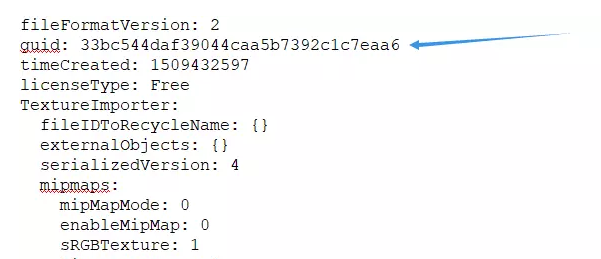
\includegraphics[scale=1]{guid}
						\caption{GUID 演示}
					\end{figure}
			如果一个资源引用了另一个外部资源,比如一个Prefab引用了其他脚本、纹理或Prefab等,则一定会标明引用资源文件的File GUID
					\begin{figure}[H]
						\centering
						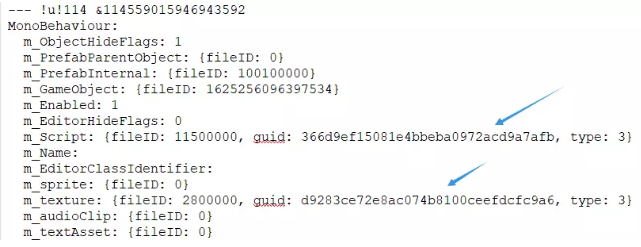
\includegraphics[scale=0.9]{guidRef}
						\caption{引用演示}
					\end{figure}
				
			\textbf{\underline{资源内部}的依赖关系}使用\verb| local ID|来确定。\textit{如果说File GUID表示为文件和文件之间的关系},那么\textbf{Local ID表示的就是文件内部各对象之间的关系},打开一个\verb|*.Prefab|文件可以很清晰的看到:
				\begin{figure}[H]
					\centering
					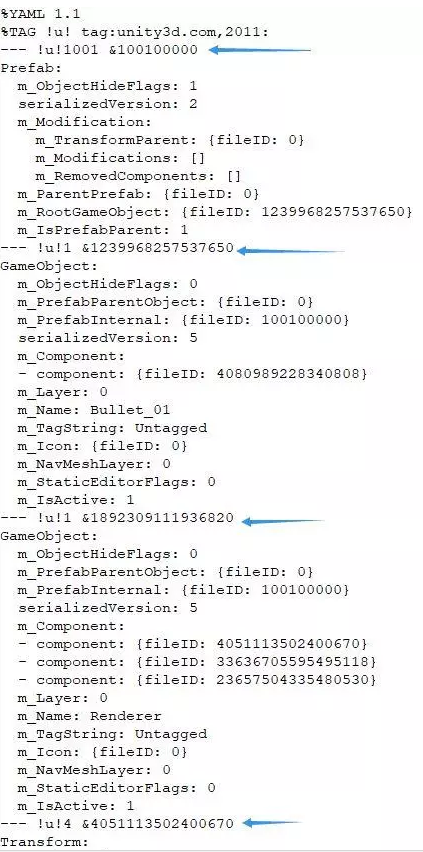
\includegraphics[scale=1.12]{localId}
					\caption{LocalId 演示}
				\end{figure}
		
			\textbf{一个对象通常是由一个或多个对象构成},每个记录在\&符号后面的数字都是一个\verb|Local ID|,每一个\verb|Local ID|也表示这它将来也会被实例化成一个对象。也就是说,当一个prefab文件要实例化成一个GameObject时,它会自动尝试获取其内部\verb|Local ID|所指的那个对象。如果这个所指的对象当前还没有被实例化出来,那么Unity会自动实例化这个对象,如此递归,直到所有涉及的对象都被实例化。
			
		\subsection{InstanceID}
			 Unity为了在运行时,提升资源管理的效率,会在内部维护一个缓存表,负责\textbf{将文件的GUID与fileID转换成为整数数值},这个数值在本次会话中是唯一的,\textbf{称作实例ID(InstanceID)}。
				
			 Unity通过\textbf{Instance ID},\textbf{来获取或判断一个对象是否已经被加载完毕}。
			
			 每当Unity读入一个\textbf{File GUID和LocalID}时,就会自动将其转换成一个简单好记的数字牌,\textit{因为通过File GUID和Local ID定位资源的效率并没有直接解引用一个地址那么快}。
			 
			 \color{blue}\textbf{如果发现这个牌上并没有挂着一把钥匙,表示当前这个这个资源还在磁盘中,尚不在内存里(没有加载);相反,如果这个牌子上有一把钥匙,表示这个资源已经被加载完毕,你可以快速的找到并使用它。}\color{black}
			 
			 Unity会在项目启动后,创建并一直维护一张“\textbf{映射表}”,这张映射表记录的就是\textbf{File GUID、Local ID}以及由它们转换而成的\textbf{Instance ID}之间的关系,\textbf{这样下次在请求资源时就可以快速的通过查看钥匙牌来获取资源了}
			 
			 \textit{程序启动时,实例ID缓存与所有工程内建的对象(例如在场景中被引用),以及Resource文件夹下的所有对象,都会被一起初始化。如果在运行时导入了新的资源,或从AssetBundle中载入了新的对象,缓存会被更新,并为这些对象添加相应条目。实例ID仅在失效时才会被从缓存中移除,当提供了指定文件GUID和fileID的AssetBundle被卸载时会产生移除操作}。
					
			 \textit{卸载AssetBundle会使实例ID失效,实例ID与其文件GUID和fileID之间的映射会被删除以便节省内存。重新载入AssetBundle后,载入的每个对象都会获得新的实例ID。}
			 
			 Unity维护的一套将GUID和LocalID解析为数据源地址的机制,这套机制中的信息,来自于:
			 	\begin{itemize}
			 		\item \textbf{场景加载时},Unity收集了与\textbf{该场景关联的}资源信息
			 		\item \textbf{项目启动时},Unity收集了所有\textbf{Resources文件夹下的}资源信息
			 		\item \textbf{读取AssetBundle时},Unity获取了\textbf{AssetBundle文件的}头部信息(Header)
			 	\end{itemize}
			 	
		\subsection{资源的生命周期}
			Object从内存中加载或卸载的时间点是定义好的。Object有两种加载方式:\textbf{自动加载}与\textbf{外部加载}。当对象的实例ID与对象本身解引用,对象当前未被加载到内存中,而且可以定位到对象的源数据,此时对象会被自动加载。对象也可以外部加载,通过在脚本中创建对象或者调用资源加载API来载入对象(例如:AssetBundle.LoadAsset) 
			
			对象加载后,Unity会尝试修复任何可能存在的引用关系,通过将每个引用文件的GUID与FileID转化成实例ID的方式。一旦对象的实例ID被解引用且满足以下两个标准时,对象会被强制加载:
			
	        实例ID引用了一个没有被加载的对象。
			
	        实例ID在缓存中存在对应的有效GUID和本地ID。
			
	        如果文件GUID和本地ID没有实例ID,或一个已卸载对象的实例ID引用了非法的文件GUID和本地ID,则引用本身会被保留,但实例对象不会被加载。在Unity编辑器中表现为空引用,在运行的应用中,或场景视图里,空对象会以多种方式表示,取决于丢失对象的类型:网格会变得不可见,纹理呈现为紫红色等等。
	        
		\subsection{MonoScripts}
			一个MonoScripts含有三个字符串:\textit{程序库名称,类名称,命名空间}。 
			
			构建工程时,Unity会收集\textbf{Assets文件夹}中\textbf{独立的脚本文件}并编译他们,\textbf{组成一个Mono程序库}。Unity会将Assets目录中的语言分开编译,\textbf{Assets/Plugins目录}中的脚本\textbf{同理}。\textit{Plugin子目录之外的C\#脚本会放在Assembly-CSharp.dll中}。而Plugin及其子目录中的脚本则放置在\textit{Assembly-CSharp-firstpass.dll}中。 
			
			这些程序库会被MonoScripts所引用,并在程序第一次启动时被加载。
	
	\section{资源文件夹}	
		\url{https://blog.csdn.net/Yao_jianlun/article/details/94839024}
		
		\subsection{Assets 文件夹}
		
		    为Unity编辑器下的资源文件夹,Unity项目编辑时的所有资源都将置入此文件夹内。在编辑器下,可以使用以下方法获得资源对象:
			
	        \verb|AssetDatabase.LoadAssetAtPath("Assets/x.txt");| 
			
	        注意:\textbf{此方法只能在编辑器下使用},当项目打包后,在游戏内无法运作。参数为包含Assets内的文件全路径,并且需要文件后缀。 
			
	        \color{blue}\textbf{Assets下的资源除特殊文件夹内,或者在会打入包内的场景中引用的资源,其余资源不会被打入包中}。\color{black}
	        
		\subsection{Resources 文件夹}
			\paragraph{资源载入}\verb|->|
			
				Assets下的特殊文件夹,\textbf{此文件夹内的资源将会在项目打包时,全部打入包内},并能通过以下方法获得对象:

					\verb|Resources.Load("fileName");|
					
		        注意:\textbf{函数内的参数为相对于Resource目录下的文件路径与名称},\textit{不包含后缀}。Assets目录下可以拥有任意路径及数量的Resources文件夹,在运行时,Resources下的文件路径将被合并。
					
		        例:\verb|Assets/Resources/test.txt|与 \verb|Assets/TestFloder/Resources/test.png|在使用\textit{Resource.Load("test")}载入时,\textit{将被视为同一资源,只会返回第一个符合名称的对象}。如果使用\textit{Resource.Load(“test”)}将返回\textit{text.txt};
					
		        如果在\verb|Resources|下有\textbf{相同路径及名称的资源},使用以上方法只能获得第一个符合查找条件的对象,使用以下方法能\textbf{获得到所有符合条件的对象}:
					\begin{lstlisting}
	Object[] assets = Resources.LoadAll("fileName");
	TextAsset[] assets = Resources.LoadAll("fileName");
					\end{lstlisting}
				 		 
			
			\paragraph{相关机制}\verb|->|
				
				在工程进行打包后,Resource文件夹中的资源将进行加密与压缩,\textbf{打包后的程序内将不存在Resource文件夹},\textbf{故无法通过路径访问以及更新资源}。
				
				在程序启动时会为Resource下的所有对象进行初始化,构建实例ID。随着Resource内资源的数量增加,此过程耗时的增加是非线性的。故会出现程序启动时间过长的问题,请密切留意Resource内的资源数量。

			\paragraph{资源卸载}\verb|->|	
					
				所有实例化后的\verb|GameObject| 可以通过\verb|Destroy|函数销毁。请留意\verb|Object|与\verb|GameObject|之间的区别与联系.
				
				\verb|Object|可以通过\verb|Resources|中的相关\verb|Api|进行卸载
					\begin{lstlisting}
	Resources.UnloadAsset(Object);//卸载对应Object 
	Resources.UnloadUnusedAssets();//卸载所有没有被引用以及实例化的Object
					\end{lstlisting}

				注意以下情况:
					\begin{lstlisting}
	Object obj = Resources.Load("MyPrefab"); 			
	GameObject instance = Instantiate(obj) as GameObjct; 
	...... 
	Destroy(instance); 
	Resources.UnloadUnusedAssets(); 
					\end{lstlisting}
					
				此时\verb|UnloadUnusedAssets|将不会生效,因为\verb|obj|依然引用了\verb|MyPrefab|,需要将\verb|obj = null|,才可生效。

		\subsection{StreamingAssets 文件夹}
			\paragraph{简介}\verb|->|
			
				\verb|StreamingAssets|文件夹为\textbf{流媒体文件夹},此文件夹内的资源将\underline{\textbf{不会经过压缩与加密}},\textbf{原封不动的打包进游戏包内}。在游戏安装时,StreamAssets文件件内的资源将根据平台,移动到对应的文件夹内。\verb|StreamingAssets|文件夹在Android与IOS平台上为\textbf{只读文件夹}. 
				
				你可以使用以下函数获得不同平台下的StreamingAssets文件夹路径:
				
					\verb|Application.streamingAssetsPath| 
				
				 请参考以下各平台下StreamingAssets文件夹的等价路径,\verb|Application.dataPath|为程序安装路径。Android平台下的路径比较特殊,请留意此路径的前缀,在一些资源读取的方法中是不必要的(\textit{AssetBundle.LoadFromFile},下详)
				
					\begin{itemize}
						\item Application.dataPath+"/StreamingAssets"//Windows OR MacOS
						\item Application.dataPath+"/Raw" //IOS
						\item "jar:file://"+Application.dataPath+"!/assets/" //Android 
					\end{itemize}
				 
			\paragraph{文件读取}\verb|->|
				
				\verb|StreamingAssets|文件夹下的文件在游戏中\textbf{只能通过}\verb|IO Stream|或者\verb|WWW|的方式\textbf{读取}(AssetBundle除外).
				\subparagraph{IO Stream 方式}\verb|->|
					\begin{lstlisting}
	using
	(
		FileStream stream = 
		File.Open(Application.streamingAssetsPath+"fileName", FileMode.Open)
	) 
	{ 
		//处理方法 
	} 
					\end{lstlisting}
				
				\subparagraph{WWW 方式}\verb|->|
					\begin{lstlisting}
	using
	(
		WWW www = 
		new WWW(Application.streamingAssetsPath+"fileName")
	) 
	{ 
		yield return www; 
		www.text; 
		www.texture; 
	} 
					\end{lstlisting}
				
				\subparagraph{AssetBundle 特有读取方式}\verb|->|
					\begin{lstlisting}
	string assetbundlePath = 
	#if UNITY_ANDROID 
		Application.dataPath+"!/assets"; 
	#else 
		Application.streamingAssetsPath; 
	#endif  
	AssetBundle.LoadFromFile(assetbundlePath+"/name.unity3d"); 
					\end{lstlisting}
					
			\paragraph{PersistentDataPath}\verb|->|
			
				\verb|Application.persistentDataPath |
				
				Unity指定的一个可读写的外部文件夹,该路径因平台及系统配置不同而不同。可以用来保存数据及文件。该目录下的资源不会在打包时被打入包中,也不会自动被Unity导入及转换。该文件夹只能通过IO Stream以及WWW的方式进行资源加载。
			
	\section{WWW 载入资源}
		\paragraph{简介}\verb|->|
			
			 WWW是一个\underline{Unity封装}的\textbf{网络下载模块},支持\textbf{Http}以及\textbf{ftp}两种URL协议,\textit{并会尝试将资源转换成Unity能使用的AssetsComponents(如果资源是Unity不支持的格式,则只能取出byte[])}。WWW加载是\textbf{异步方法}。
				\begin{lstlisting}
	byte[] bytes = WWW.bytes; 
	string text = WWW.text; 
	Texture2D texture = WWW.texture; 
	MovieTexture movie = WWW.movie; 
	AssetBundle assetbundle = WWW.assetBundle; 
	AudioClip audioClip = WWW.audioClip; 
				\end{lstlisting}
			
		\paragraph{相关机制}\verb|->|
			
			每次new WWW时,Unity都会启用一个线程去进行下载。通过此方式读取或者下载资源,会在内存中生成WebStream,WebStream为下载文件转换后的内容,占用内存较大。使用WWW.Dispose将终止仍在加载过程中的进程,并释放掉内存中的WebStream。 
			
	        如果WWW不及时释放,将占用大量的内存,推荐搭配using方式使用,以下两种方式等价。
	        \subparagraph{通过new WWW、Try}:
				\begin{lstlisting}
// 方式一			
WWW www = new WWW(Application.streamingAssetsPath+"fileName"); 
try 
{ 
	yield return www; 
	www.text; 
	www.texture; 
} 
finally 
{ 
	www.Dispose(); 
} 
				\end{lstlisting}
			
			\subparagraph{通过Using}:	
				\begin{lstlisting}
// 方式二
using(WWW www = 
	new WWW(Application.streamingAssetsPath+"fileName")) 
{ 
	yield return www; 
	www.text; 
	www.texture; 
} 	
				\end{lstlisting}
			
			如果载入的为Assetbundle且\textbf{进行过}压缩,则\textbf{还会在}内存中\textbf{占用一份}AssetBundle解压用的缓冲区\textit{Deompresion Buffer}, \textbf{AssetBundle}压缩格式的不同会影响此区域的大小。
			
		\paragraph{LoadFromCacheOrDownload}\verb|->|
			
			\begin{lstlisting}
	int version = 1; 
	WWW.LoadFromCacheOrDownload(PathURL+"/fileName",version); 
			\end{lstlisting}
			
	       使用此方式加载,将\textbf{先从硬盘}上的存储区域\textbf{查找是否有对应的资源},\textbf{再验证本地}Version与传入值之间的关系,如果传入的Version\textbf{大于}本地,\textit{则从传入的URL地址下载资源,并缓存到硬盘,替换掉现有资源},如果传入Version\textbf{小于等于}本地,\textit{则直接从本地读取资源};\textbf{如果本地没有存储资源,则下载资源}。
	       
	       \color{blue}此方法的存储路径无法设定以及访问。使用此方法载入资源,不会在内存中生成 WebStream(其实已经将WebStream保存在本地),如果硬盘空间不够进行存储,将自动使用new WWW方法加载,并在内存中生成WebStream。在本地存储中,使用fileName作为标识符,所以更换URL地址而不更改文件名,将不会造成缓存资源的变更。 	
		   保存的路径无法更改,也没有接口去获取此路径\color{black}
			
	\section{AssetBundle}	
		\url{https://blog.csdn.net/qq_35361471/article/details/82854560}
	
		\subsection{工作流程}
			\dirtree{%
				.1 \textbf{AssetBundle 的使用流程} . 
				.2 1- 创建AssetBundle .
				.3 2- 上传到Server .
				.4 3- 游戏运行时根据需要下载AssetBundle 文件 .
				.5 4- 解析加载Assets .
				.6 5- 使用完后释放内存等资源 .
			}
			
			\paragraph{图例}AssetBundle 资源组织形式:
				\begin{figure}[H]
					\centering
					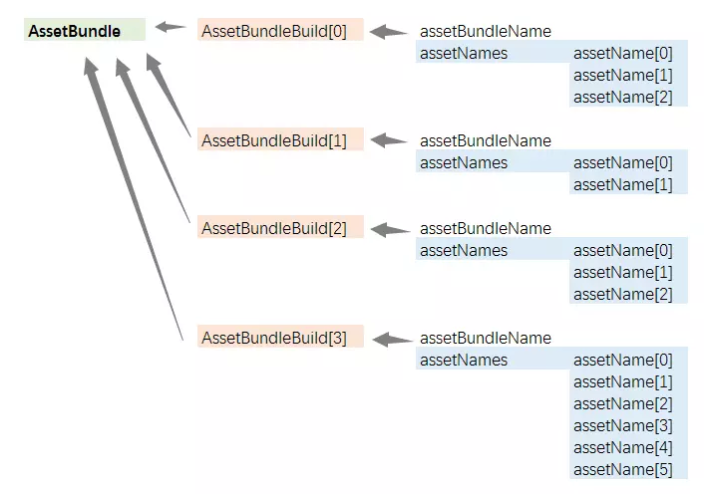
\includegraphics[scale=0.7]{AssetBundle}
					\caption{AssetBundle 组织形式}
				\end{figure}
		
		\subsection{关键路径说明}
			\paragraph{Resources -只读}
				\begin{itemize}
					\item Resources文件夹下的资源无论使用与否都会被打包
					\item 资源会被压缩,转化成二进制
					\item 打包后文件夹下的资源只读
					\item 无法动态更改,无法做热更新
					\item 使用\verb|Resources.Load|加载
				\end{itemize}
				
			\paragraph{StreamingAssets -只读}
				\begin{itemize}
					\item 流数据的缓存目录
					\item 文件夹下的资源无论使用与否都会被打包
					\item 资源不会被压缩和加密
					\item 打包后文件夹下的资源只读,主要存放二进制文件
					\item 无法做热更新
					\item WWW类加载(一般用CreateFromFile ,若资源是AssetBundle,依据其打包方式看是否是压缩的来决定)
					\item 相对路径,具体路径依赖于实际平台
				\end{itemize}
				
			\paragraph{Application.dataPath -只读}
				\begin{itemize}
					\item 游戏的数据文件夹的路径(例如在Editor中的Assets)
					\item 无法做热更新
					\item 很少用到
				\end{itemize}
			
			\paragraph{Application.persistentDataPath -读写}
				\begin{itemize}
					\item 持久化数据存储目录的路径( 沙盒目录,打包之前不存在 )
					\item 文件夹下的资源无论使用与否都会被打包
					\item 运行时有效,可读写
					\item 无内容限制,从StreamingAsset中读取二进制文件或从AssetBundle读取文件来写入PersistentDataPath中
					\item 适合热更新
				\end{itemize}
		
		\subsection{热更新原理}
			\dirtree{%
				.1 .
				.2 将\textbf{StreamingAsset目录}下的文件,\textbf{全部复制}到目标平台(ios/Android)的\textbf{数据目录}中(第一次运行游戏时) .
				.3 启动游戏前刷新所有文件夹,\textit{客户端文件}与\textit{服务上的文件}\textbf{对比MD5},\textbf{记录不同的文件,下载对应的文件替换} .
				.4 从数据目录加载AB(使用协程不使用线程) .
				.5 实例化后卸载内存中的AB .
			}
				
		
			\url{https://www.cnblogs.com/fuyunzzy/p/6527120.html}
		
			\begin{figure}[H]
				\centering
				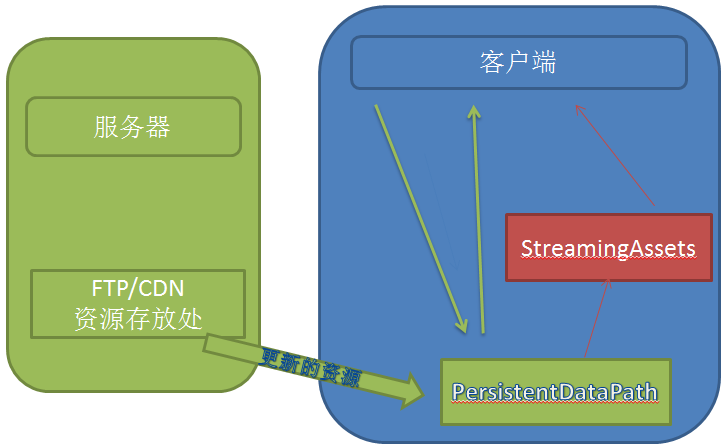
\includegraphics[scale=0.45]{AbUpdate}
				\caption{热更目录关系}
			\end{figure}
			
			\begin{figure}[H]
				\centering
				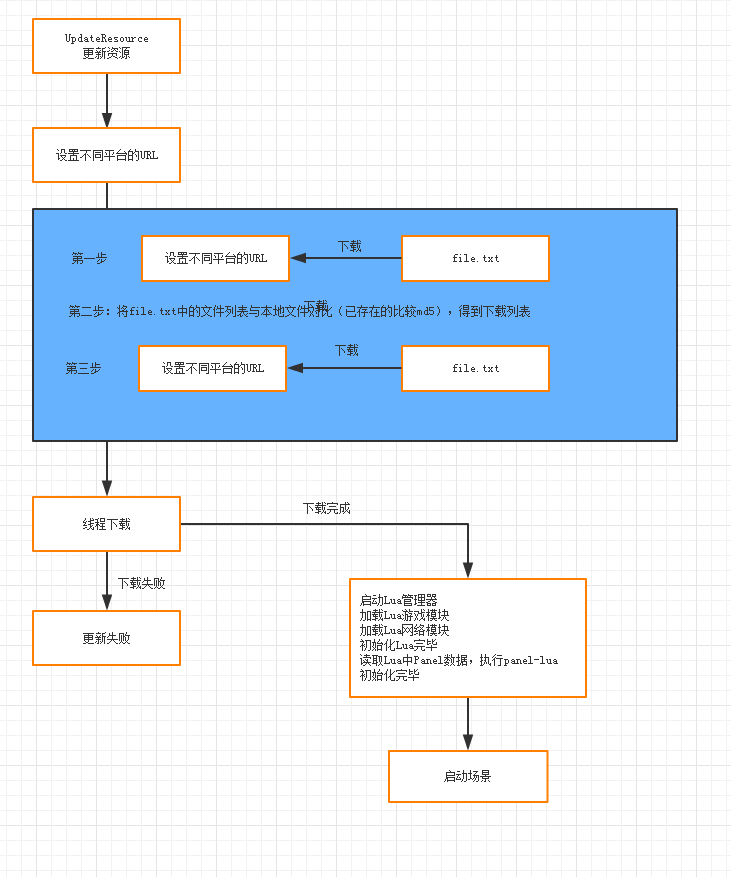
\includegraphics[scale=0.5]{AbUpdateProcess}
				\caption{热更流程}
			\end{figure}			
			
			
			\paragraph{Notice}加载(和下载)AB的思路
				\begin{itemize}
					\item 建立一个队列,队列中有加载AB的请求时,去加载,加载完成后移出队列,加载下一个直到完成
					\item Unity5.0之后的AB资源是分开的,加载时难以判断依赖关系,而且AB资源在内存中只能有一个,所以\textbf{使用单线程加载}
				\end{itemize}
		\subsection{AB包之间的关系}
			\begin{figure}[H]
				\centering
				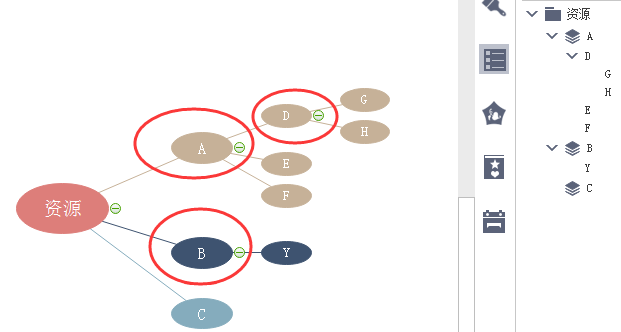
\includegraphics[scale=0.64]{AbRelative}
				\caption{AB 包依赖关系说明}
			\end{figure}
			
			画红圈的就是有依赖关系的,在Unity中,如何知道有哪些资源有依赖关系呐。	
			
			一般,我们每次Build后会\textbf{自动生成AndroidManifest.xml},这里面就详细叙述了资源之间的依赖关系。
			
			\subsubsection{AssetBundle之间的依赖}	
			
				如果游戏中的某个资源被多个资源引用(例如游戏中的Material),单独创建AssetBundle会使多个AssetBundle都包含被引用的资源(这里跟flash编译选项中的链接选项有些像),从而导致资源变大,这里可以通过指定AssetBundle之间的依赖关系来减少最终AssetBundle文件的大小(把AssetBundle解耦)。
								
				具体方法是在创建AssetBundle之前调用BuildPipeline.PushAssetDependencies和BuildPipeline.PopAssetDependencies来创建AssetBundle之间的依赖关系,它的用法就是一个栈,后压入栈中的元素依赖栈内的元素。
		
			\subsubsection{加载依赖关系}
				\begin{lstlisting}
	 AssetBundle _manAB = AssetBundle.LoadFromFile(_manpath);
     //固定格式
     AssetBundleManifest manifest = _manAB.LoadAsset<AssetBundleManifest>("AssetBundleManifest");
     string[] dependencies = manifest.GetAllDependencies(ABName);
				\end{lstlisting}
				
		\subsection{创建}
			通过编译管线BuildPipeline来创建AssetBundle文件,总共有三种方法,具体如下所示。
			\subsubsection{BuildAssetBundle}
				该API将编辑器中的任意类型的Assets打包成一个AssetBundle,适用于\textbf{对单个大规模场景的细分}。
				
				\textit{每一次调用BuildPipleLine.BuildAssetBundles时},\textbf{将会生成一批AssetBundle文件},具体数量根据传递AssetBundleBuild数组决定,\textbf{每一个AssetBundleBuild对象将对应\textit{一个AssetBundle}及\textit{一个同名+.manifest后缀文件}}。其中AssetBundle文件的后缀用户自行设置,比如".unity3d",".ab"等等;而\verb|.manifest|文件是给人看的,\textbf{里面有这个AssetBundle的基本信息以及非常关键的资源列表}。
				
				除了AssetBundleBuild数组所定的AssetBundle外,\textit{还将额外在output路径下生成的一对与output文件夹同名的文件及一个同名.manifest后缀文件}。\textbf{这个同名文件可厉害了,它记录了这批次AssetBundle之间的相互依赖关系}。\textit{当然.manifest文件还是给人看的,我们可以用它分析资源间的依赖关系,但是在项目实际运行时,Unity并不会关心它。}
				
					\begin{figure}[H]
						\centering
						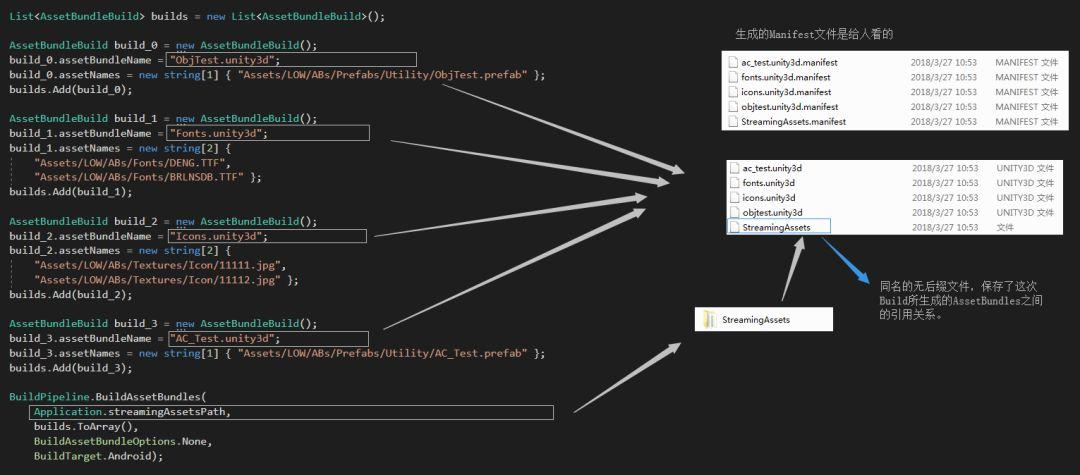
\includegraphics[scale=0.54]{AssetBuild}
						\caption{BuildAssetBundles示例}
					\end{figure}
				
			\subsubsection{BuildStreamedSceneAssetBundle}
				该API将一个或多个场景中的资源及其所有依赖以流加载的方式打包成AssetBundle,一般适用于\textbf{多单个或多个场景进行集中打包}
				
				
			\subsubsection{BuildAssetBundleExplicitAssetNames}
				该API功能与a相同,但创建的时候可以为每个Object指定一个自定义的名字。(一般不太常用)
				
		\subsection{下载方式}
			通过对比persistencePath 下的AB下的version 文件,决定需要下载什么。
			\begin{figure}[H]
				\centering
				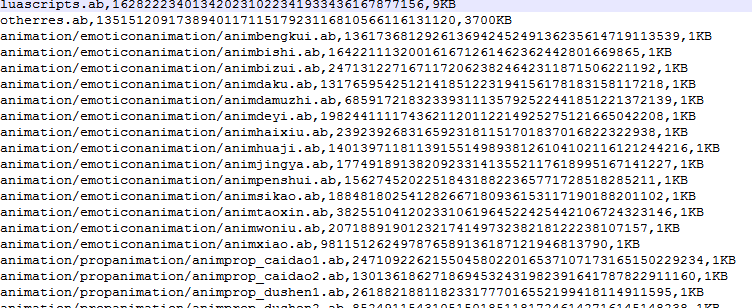
\includegraphics[scale=0.45]{AbDownload}
				\caption{AbDownload 方式}
			\end{figure}
		
		\subsection{AssetBundle压缩类型}
			\begin{itemize}
				\item 不压缩
				\item LZMA
				\item LZ4
			\end{itemize}	
			
			\subsection{LZMA 与 LZ4压缩对比}
				假如你是一个Prefab,妹纸是一个资源,妹纸在一个闺蜜圈.你想约妹纸出来吃饭
			
				LZ4:直接约妹纸出来就可以了,\textbf{块读取}
			
				LZMA:首先要通知整个闺蜜圈,然后再看圈内人跟其他圈子会有什么关系,把相关人也一起通知(闺蜜丈夫等)然后闺蜜丈夫再找相关关系人,直到全部都批准了,才能和妹纸吃饭.(\textbf{依赖读取}),Android.manifest包含了AB资源的信息(名称,依赖等),可以使用AssetDatabase.GetDependencies(path),找出资源引用关系
				

				LZMA会比LZ4读取成本高不少,特别是在Assetbundle包引用混乱的情况下
				
				
			\subsection{选择策略}
				
				
		\subsection{加载方式}   
			根据AssetBundle文件所在的位置(本地、远端),AssetBundle有不同的加载方式,一般可以分为以下4种。
			\begin{itemize}
				\item WWW
				\item LoadFromFile 或 LoadFromFileAsync
				\item WebRequest
				\item LoadFromMemory
			\end{itemize} 
			
			\textbf{AssetBundle的加载}可以理解为:\textbf{Bundle加载}和\textbf{Asset加载}两部分。因为AssetBundle文件可以从功能上分为两大块:
			\begin{enumerate}
				\item Header 部分:记录文件标记、压缩信息、文件列表
				\item Data 部分:记录资源实际内容
			\end{enumerate}
			
			当使用\textit{AssetBundle.LoadFromFile}或\textit{LoadFromFileAsync}时,在pc平台及移动平台上,unity\textbf{仅会为我们读取AssetBundle的header部分,并不会将bundle的data部分整个读入内存}。
			
			\textbf{当调用上一步生成的AssetBundle对象读取具体资源时}(\textit{LoadAsset, LoadAssetAsync, LoadAllAssets}),Unity会参考已经缓存的文件列表,\textbf{找到目标资源在data部分的位置并读入到内存中}。

			如果一个资源引用到了其他资源,则必须要先读入被引用资源的AssetBundle文件,否则就会发生引用Miss。
			
			为了避免上面Miss的情况,在加载资源时,首先需要将该资源的依赖项全部加载完毕,不过仅需加载依赖资源的AssetBundle文件。也就是说,我们只要将该依赖AssetBundle的Header部分加载(AssetBundle.LoadFromFile或LoadFromFileAsync)就可以,这样在真正读取Asset时,Unity会自动处理好真实依赖的Asset,我们不用操心。
			
			AssetBundle的依赖关系如何读取呢?加载上面提到的那个很厉害的文件就可以了。
				\begin{lstlisting}
	// 用与读取AssetBundle 一样的方式读取AssetBundleManifest
	var bundle = AssetBundle.LoadFromFile(bundleManifestPath);
	if(bundle)
	{
		// 读取AssetBundleManifest 资源
		AssetBundleManifest abManifest = bundle.LoadAsset<AssetBundleManifest>("AssetBundleManifest");
		// 获取生命的全部AssetBundle, 对应一次BuildPipeline.BuildAssetBundles
		string[] assets = abMainifest.GetAllAssetBundles();
		// 遍历所有AB 资源
		foreach(var item in assets)
		{
			// 获取AB资源的直接依赖 A->B->C 则返回B
			string[] dependencies = abManifest.GetDirectDependencies(item);
			// 获取AB 资源的所有依赖资源 A->B->C 则返回BC
			// string[] dependencies = abManifest.GetAllDependencies(item);
		}
	}
				\end{lstlisting}
				
				
				
				
		\subsection{加载优先级}		
			\textbf{首先}加载的是 \textbf{常驻公共资源},
			
			\textbf{再}加载经常\textbf{反复资源},
			
			当然如果进入战斗(某个\textbf{特定模块}),就加载\textbf{非常驻公共资源}。
			
			\textbf{其他资源是当使用时加载}。	

		
		\subsection{缓存}
			一般常驻资源,最好\underline{缓存}\textbf{把AB存为需要的GameObject},例如子弹之类。

		\subsection{使用}
			当\verb|AssetBundle|被成功加载后,调用该\verb|Assebbundle|对象的\verb|LoadAsset|、\verb|LoadAllAssets|或对应的异步版本即可加载资源,也就是实例化对象。\textbf{如果这个对象已经被加载过,Unity并不会重复加载},还记得之前所说的映射表么,被加载过的资源就好比挂上了数字牌的钥匙,直接对地址解引用即可。
			
			\begin{table}
				\centering
				\caption{AssetBundle 加载方式对比}
				\begin{tabular}{p{5cm}<{\centering}|p{3cm}<{\centering}|p{3cm}<{\centering}|p{3cm}<{\centering}}
					\toprule
						方式 & 不压缩 & LZ4 & LZMA\\
					\midrule
						WWW 加载 & & & \\
						LoadFromCacheOrDownload 加载 & & & \\
						LoadFromMemory (异步)加载 & & & \\
						LoadFromFile(异步)加载 & & & \\
						WebRequest 加载 & & & \\
					\bottomrule
				\end{tabular}
			\end{table}
		\subsection{释放资源-卸载}
			常驻资源肯定是不能unload(false)的,这边释放资源,释放的是其他资源。
			
			对于unload(false),还是unload(true). unload(false)适合反复使用资源,一次Load之后,再也不需要Load,\textbf{且与其他资源没有"被依赖关系"}。
			
			\begin{itemize}
				\item \verb|unload(false)|,释放的是自身。
				\item \verb|unload(true)|,释放的是自身以及自身所有的子节点。因此,unload(true),慎用。
			\end{itemize}
		
		\subsection{内存模型}
			\begin{figure}[H]
				\centering
				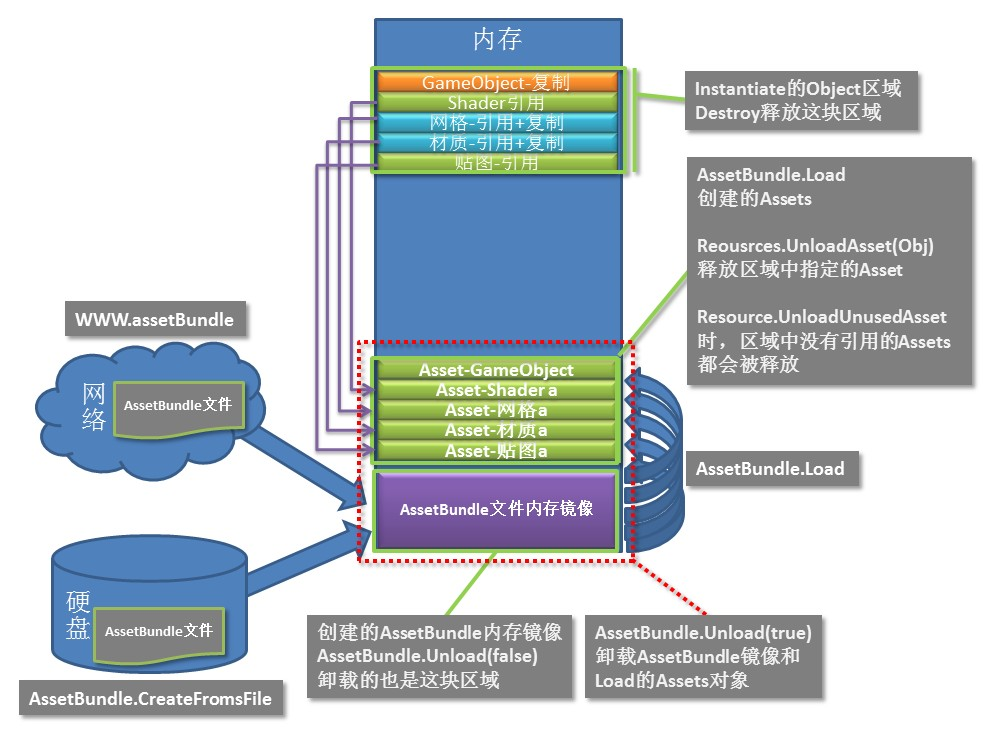
\includegraphics[scale=0.7]{assetBundel}
				\caption{AssetBundle 内存模型}
		\end{figure}
		
	\section{资源打包}
		Unity  以下资源会被打进包里。
		\begin{itemize}
			\item Assets下所有脚本
			\item Assets下所有被引用到的所有文件
			\item Resource下的所有文件
			\item Plugins下的对应平台下的所有文件
			\item StreamingAssets下的所有文件
			\item AB包打成大包的时候会打进包体
		\end{itemize}
	
	
		打包成功后,没有在特殊目录的文件都会打到Resource 中,而Resource 中的资源都会引用一份目前的文件副本,所以如果引用的热更资源、但是本身又被打入Resource,那么热更是不起作用的。
		
		\subsection{降低包体准则}
			\begin{itemize}
				\renewcommand\labelitemi{\makebox[0pt][l]{$\square$}\raisebox{.15ex}{\hspace{0.1em}$\checkmark$}}
				\item 打包Android 可以选择sdk版本不用太高
				\renewcommand\labelitemi{\makebox[0pt][l]{$\square$}\hspace{1em}}
				\item 在StreamingAssets删除不用的东西
				\item 打包时查看log纪录,由此判断需要减少的文件类型
				\item 优化,压缩网格和动画,减少文件大小
				\item 优化,压缩图片,减少图片大小
				\item 剔除教程:\url{https://blog.csdn.net/yxriyin/article/category/2879081}
					\begin{itemize}
						\item 分析打包的日志文件删除无用文件
						\item 重制图集
						\item 压缩png
						\item 剔除重复资源
					\end{itemize}
			\end{itemize}
		
			针对于目前这种困境,不少的服务商推出了分包技术,而传统的分包是将资源切割,分段下载,进入游戏前进行二次下载;处理游戏包体瘦身时,往往采用删除代码,精简资源甚至作资源取舍的方式;在资源加载时,玩家必须要中断游戏,并在等待中进行缓慢的资源加载。
			
			官方解释对我们帮助甚少。所以,我们还需要一样利器,\verb|www.LoadFromCacheOrDownload|。我把包分成三段:
				\begin{enumerate}
					\item \textbf{首包}(里面包含了最最必要的资源)。
					\item \textbf{首次进入包加载}(加载游戏运行必要的资源)。
					\item \textbf{游戏运行中资源加载}(按每个游戏不同各自定义,以场景和单位个体为主要,在画面进入时加载资源,加载结束后再运行并显示)。
				\end{enumerate}
			
			
		\subsection{针对删除无用资源的方案}
			\url{https://www.cnblogs.com/alongu3d/p/3203292.html}
			
			\url{https://github.com/handcircus/Unity-Resource-Checker}
			
			
			
			
			
	\section{参考}
		\url{https://blog.csdn.net/swj524152416/article/details/54022282}
		
		\url{https://blog.csdn.net/foxyfred/article/details/73995577}
		
		\url{https://www.jianshu.com/p/2a7c4a48aaee}
		
		\url{http://www.360doc.com/content/17/1130/11/50169787_708566648.shtml}
		
		\url{https://docs.unity3d.com/Manual/ReducingFilesize.html}
\chapter{Editor 扩展}
	Unity编辑器扩展是扩展Unity菜单功能,也可以说是自定义Unity菜单,以此来便利我们能够更快捷地开发游戏。
	\section{流程}
		\begin{enumerate}
			\item 在Asset文件夹下\textbf{创建一个文件夹}\verb|Editor|,如果已经存在则忽略此步
			\item 在\verb|该Editor| 文件夹下,\textbf{创建一个}\verb|C#|\textbf{脚本},无需继承于任何类
			\item \textbf{引用}\verb|UnityEditor| \textbf{命名空间}
			\item \textbf{写静态方法}\textit{既菜单的功能},类似于\verb|[SerilizedFiled]|下的东西,与\verb|[Menuitem("Netease/xx")]|一一对应。
			\item \textbf{给该方法上添加}\verb|[Menuitem("")]|特性
		\end{enumerate}	
	
	\section{在编辑器上增加一个MenuItem}
	
	
	\section{创建一个对话框}
	
	
	\section{扩展Inspector面板}
	
	
	
	\section{编辑器插件常用函数}
		\subsection{资源导入回调函数}
			当导入资源到Unity 项目中的某个资源文件夹下时,当Unity Editor获得焦点后,会在加载完资源后,先为其创建.meta 文件,然后再触发该回调函数。
			
			\begin{lstlisting}[frame=line]
	public class TestBundleNameAndTexture : UnityEditor.AssetPostprocessor
	{
	    static void OnPostprocessAllAssets(  // 这个函数必须为静态的,其他可以不是!
	        string[] importedAssets,
	        string[] deletedAssets,
	        string[] movedAssets,
	        string[] movedFromAssetPaths)
	    {
	        foreach (var path in importedAssets)
	        {
	            DirectoryInfo dir = new DirectoryInfo(path);
	            Debug.Log(dir.Parent.FullName);
	            BundelNameCreater.Proc(dir.Parent.FullName);
	        }
	    }
	
	}
			\end{lstlisting}
	\section{一些常用的Inspector属性设置}
	
	
	\section{参考}
		\url{https://blog.csdn.net/puppet_master/article/details/51012298}
		
		\url{http://blog.csdn.net/asd237241291/article/details/38235091}
		
		\url{http://blog.sina.com.cn/s/blog_471132920101n8cr.html}
		
\chapter{跨平台发布apk}
	\section{操作流程}
		\begin{itemize}
			\item 安装 JavaSDK、Android Studio 并在SDK manager 里添加对应的API包
			\item 在unity 中的\verb|edit |选项下的\verb|preferences|, 并选中\verb|External Tools| 选项,配置\verb|JDK |和\verb|Android SDK| 安装位置。
			\item 在unity 中的\verb|File -> Build Settings|中,添加需要添加的场景,并选择对应的平台(Android, IOS)等
			\item 在unity 中的\verb|Build Settings |中的\verb|Player Settings |设置以下几个重要内容。
				\begin{enumerate}
					\item \verb|Company Name |
					\item \verb|Product Name |
					\item \verb|Default Icon |:192$\times$192
					\item \verb|Default Orientation |
					\item \verb|Other Settings -> Identification |:修改为\verb|com.netease(Or Other).TestName(Or Other)|
				\end{enumerate}
		\end{itemize}	
	
	\section{Apk 安装常见错误}
		\url{http://mumu.163.com/2017/03/30/25905_680657.html}

	

\chapter{AI}
	Most game AI that currently exists is hand coded, consisting of decision-trees with sometimes up to thousands of rules. All of which must be maintained by hand, and thoroughly tested. In contrast, ML relies on algorithms which can make sense of raw data, without the need of an expert to define how to interpret that data.
	
	This automated learning can be applied specifically to game agent behavior a.k.a. NPCs. We can use Reinforcement Learning (RL) to train agents to estimate the value of taking actions within an environment. 
	
	\section{行为树}
		
	
	\section{Machine Learing}
		\url{https://blogs.unity3d.com/2017/09/19/introducing-unity-machine-learning-agents/?_ga=2.160895102.2116653917.1574651205-1790393125.1531538815}

		
		\subsection{BanditDungeon}
			\url{https://github.com/Unity-Technologies/BanditDungeon}
			
			\url{https://blogs.unity3d.com/2017/06/26/unity-ai-themed-blog-entries/}
			
			在最简单的情况下,有一个包含两个箱子的房间。打开箱子会产生钻石(好东西)或鬼(坏东西)。多次打开相同的箱子会根据产生钻石的一些潜在概率产生不同的钻石和幻影序列。例如,概率为0.5的胸部表示将产生50-50的钻石和鬼影的混合,而概率为0.9的胸部则表示将产生十分之一的钻石(约十分之一)。注意,每个箱子都有其自己的真实概率,该主体(在这种情况下,是决定打开哪个箱子的实体)不知道的。代理人每次选择箱子时,在发现钻石的情况下要么获得正面奖励,要么在发现鬼影的情况下获得负面奖励。代理商的目标是在许多试验中最大化其总奖励-在每次试验中,代理商都可以选择任何箱子。
			
			如果探员知道每个箱子的真实潜在概率,那么它的任务就很简单,它要做的就是反复选择产生钻石可能性最高的箱子。但是,在没有此信息的情况下,最好的办法是在估计概率(称为探索)与选择具有最高估计概率的胸部(称为利用)之间进行明智的权衡。仅进行探索的特工将浪费所有估计每个箱子概率而不最大化其自身奖励的试验,而进行有限探索的特工将基于不准确的概率估算浪费大部分试验。这里的关键是如何有效地平衡勘探与开发。
			
			包含两个箱子的单个房间的最简单方案可以扩展为包括多个箱子的多个房间。在此演示中,您将可以在无状态的强盗(一个房间)或上下文的强盗(三个房间)之间进行选择。对于这两种情况中的任何一种,除了下面讨论的其他一些设置之外,您还可以选择每个房间的箱子数(2至5)。
			
			\textbf{最后收敛到一种策略获取到最大的Rewards.}
		
		
		\subsection{Q-GridWorld}
			\url{https://github.com/Unity-Technologies/Q-GridWorld}
			
			\url{https://blogs.unity3d.com/2017/08/22/unity-ai-reinforcement-learning-with-q-learning/}

			在最简单的情况下,我们有一个5x5的网格世界,其中有一个特工(蓝色方块),一个目标(绿色方块)和障碍物(红色方块)。对于演示的每次运行,都会随机选择代理商,目标和障碍物的位置(但在同一演示运行中保持一致)。在这种网格世界环境中,代理的目标是学习一种策略,以有效地从其起始位置导航到目标位置,同时避免障碍。它通过学习针对每个状态所采取的最佳措施来实现这一目标(通常称为强化学习中的策略)。这里的动作是移动的方向(北,南,东和西),而这里的状态是其在网格世界中的位置。从本质上讲,它学习从起始位置到目标位置的最短无障碍路径。
			
			此处实施的Q学习算法通过为每个操作状态对维护一个数值来学习策略,该数值表示在处于特定状态时采取特定操作的程度。当代理探索网格世界时,每个操作状态对的此数字值都会增量更新。直观上讲,它执行几次试验,其中试验是一系列在障碍物或目标位置结束的动作。然后,对于它在整个试验中执行的每个动作状态对,如果是肯定试验(在目标位置结束),则将其值增加;如果是否定试验(与障碍物相撞),则将其值减小。代理还鼓励其发现每一条最短路径时所采取的每一个步骤都会得到少量的负面奖励。
			
			与我们之前的多臂匪徒演示类似,这里需要进行勘探与开发的权衡。当代理程序正在进行试验时,它会在随机选择操作和在给定状态下遵循当前对最佳操作的猜测之间进行混合。这种权衡是由一个从1开始的ε参数控制的(鼓励进行全面探索),并且在整个试验过程中将其逐渐减小到0.1(限制探索)。因此,在运行演示时,您会注意到,随着演示的进行和epsilon值的下降,代理的动作变得越来越可预测,\textbf{收敛到从其起始位置到目标位置的最佳路径}。



\chapter{Unity 优化经验@实况}
	\section{加载时间}
		\begin{itemize}
			\item IO
			\item 网络请求
			\item GC
			\item 加密解密
			\item 协程等待
			\item 网格重建
			\item Mono 初始化
		\end{itemize}
	
	\section{内存分类}
		\begin{itemize}
			\item 资源内存:Texture、Sound、Material
			\item 引擎模块:Web Stream(WWW)、SerializedFile(AB)
			\item 托管堆:Class Array Container
		\end{itemize}
		
		\subsection{内存问题}
			\begin{itemize}
				\item 内存泄漏
				\item 纹理格式错误
				\item Unload
				\item 字符串操作
				\item Instantiate
				\item Linq
				\item 堆内存碎片化
			\end{itemize}
		
		\subsection{内存工具}
			\begin{itemize}
				\item Unity Profile
				\item Memory Profile
				\item IOS Instruments
			\end{itemize}	
		
		
	\section{资源缩减}
		\begin{itemize}
			\item 清除无用资源,重复资源
			\item 确定资源压缩格式
			\item 确认贴图是否开启了mipmap
			\item 确认贴图是否合理的使用了九宫格
			\item 确认大贴图是否是缩小显示了
			\item 在保证视觉效果不受太大损失的情况下,尝试减少贴图尺寸
		\end{itemize}	
		
\chapter{GC-Garbage Collection}
	介绍性:\url{https://blog.csdn.net/znybn1/article/details/76464896}
	优化减少GC:\url{https://blog.csdn.net/chenxuezhi123/article/details/45249935}
	\section{}
	
	\section{}
	
	\section{}
		

\chapter{调试技巧}
	\section{以父类为基点}
		在Inspector 中查看是否存在父类脚本\verb|[SerializedField]| 的变量,这样方便对空间进行查找,并且添加新的\textbf{控制}			
	
	
	\section{Android 与 Unity 互相调用}
		参考:\url{https://www.cnblogs.com/Colored-Mr/p/5677209.html}

		\subsection{Unity 调用 Android 非静态方法}
			\begin{lstlisting}
	// Unity 代码
	AndroidJavaClass jc = new AndroidJavaClass ("com.unity3d.player.UnityPlayer");
	AndroidJavaObject jo = jc.GetStatic<AndroidJavaObject> ("currentActivity");
	jo.Call ("login","");	
	
	// Android 代码
	public void login( String str ) {      
      // 写上自己的操作
	}
			\end{lstlisting}
		
			当我自己实际测试的时候发现,Android这边的\verb|login()|不一定要写在\textit{com.unity3d.palyer}包名下的UnityPalyer类下。
			
			你只需要把\verb|login()|写在你自己定义包名下的\textit{UnityPlayerActivity.java}中就可以了。当然了,该类肯定是继承Activity的。
			
			你可以把鼠标放在unity代码的Call上查看方法可以填写的参数, 你会发现方法可以填写的参数可以是\verb|params object[]|。也就是可以传递多个参数,以数组的形式传递给\verb|Android|。
		
		\subsection{Unity 调用 Android 静态方法}
			\begin{lstlisting}
	// Unity 代码
	public void PKBtnClick() {
	    this.test("test1", "test2", "test3", 1, true);
	}
	
	public void test( params object[] args ){
	    AndroidJavaClass jc = new AndroidJavaClass ("com.Indra.Dark.UnityPlayerActivity");
	    jc.CallStatic ("login", args);
	}
	
	// Android 代码
	public static  void login( String str1, String str2, String str3, int a, boolean isShow ) {
	    if( isShow ){            
	        Log.e("test", str1 + "==" + str2 + "==" + str3 + "==" + a );
	  }
	}
			\end{lstlisting}
			
			unity代码中"\verb|com.Indra.Dark.UnityPlayerActivity|"为真实的包名.类名,即com.Indra.Dark是\textbf{包名},UnityPlayerActivity为\textbf{类名}
				
		\subsection{Android 调用 Unity}
			\begin{lstlisting}
	UnityPlayer.UnitySendMessage("btnTest", "showLog", "a#b#c");
			\end{lstlisting}
			
			UnitySendMessage的第一个参数是unity控件的名字,第二个参数是方法名,第三个参数是要传递的参数。而且只能传递一个参数。不过你可以把你要传递的参数做成一个字符串传递过去,unity那边做分割字符串就行了。例如上面就是把a,b,c用\#连接起来。unity那边用\#作为分隔符去分割就OK了。
		
			那么问题来了,脚本挂在的unity控件名字不好找怎么办。其实还有个办法轻松搞定,那就是在脚本的Start()方法中指定name为你方法传递的控件名字就OK了。
			
			如我上面的方法中要找的控件是btnTest,则:
			\begin{lstlisting}
	void Start () {
	    this.name = "btnTest";
	}
	
	void showLog(string str){
	  Debug.Log("str:" + str );
	}
			\end{lstlisting}
	
\chapter{书籍推荐}
	
	GPU Gems:\url{https://developer.nvidia.com/gpugems/GPUGems/gpugems_ch01.html}
	
	Real Time Rendering
	
	Uniyt Shader 入门精要
	
	\section{Unity AB包 入门参考}
		\begin{itemize}
			\item 各目录关系\url{https://www.cnblogs.com/u3ddjw/p/6691932.html}
			\item AB加载 \url{https://www.cnblogs.com/u3ddjw/p/9120430.html}
			\item AB资源关系 \url{https://www.cnblogs.com/u3ddjw/p/9120430.html}
		\end{itemize}
		
\end{document} 
 		    